

\documentclass[11pt]{beamer}
\hypersetup{pdfencoding=auto}

\usetheme{Berkeley}

\usepackage{xcolor}
\usepackage{amssymb,amsmath,graphicx}
\usepackage{kotex}
\usepackage{multimedia}
\usepackage{setspace}
\usepackage{multicol}
\usepackage{verbatim} %use 

%% Color Setting %%
\definecolor{Grey}{rgb}{0.6,0.6,0.6}
\definecolor{GSHSred}{RGB}{105,0,0}
\definecolor{GSHSRED}{RGB}{80,0,0}
\definecolor{gshsred}{RGB}{240,210,210}
\setbeamercolor{title}{bg=white,fg=GSHSred}
\setbeamercolor{author}{fg=GSHSred}
\setbeamercolor{institute}{fg=GSHSred}
\setbeamercolor{date}{fg=GSHSred}
\setbeamercolor{logo}{bg=GSHSred}
\setbeamercolor{sidebar}{bg=GSHSred}
\setbeamercolor{frametitle}{bg=white,fg=GSHSred}
\setbeamercolor{section in sidebar}{use=sidebar,bg=white,fg=sidebar.bg}
\setbeamercolor{subsection in sidebar}{parent=section in sidebar}
\setbeamercolor{subsubsection in sidebar}{parent=subsection in sidebar}
\setbeamercolor{item}{fg=GSHSred}
\setbeamercolor{block title}{bg=GSHSRED,fg=white}
\setbeamercolor{block body}{bg=gshsred,fg=black}

%% Frametitle Setting %%
\setbeamerfont{frametitle}{series=\bfseries}
\setbeamertemplate{frametitle}
{ \vspace*{-10mm}
  \leavevmode
  \hspace*{3pt}
  \begin{beamercolorbox}[wd=\paperwidth,ht=1ex,dp=1ex]{frametitle}
    \hspace*{7pt}\underline{\makebox[0.6\paperwidth][l]{
    \Large{\insertframetitle}}}
  \end{beamercolorbox}
}

             
%% Title Page Setting %%
\setbeamerfont{title}{series=\bfseries}
\setbeamertemplate{title page}{
  %% Background Logo
  \begin{picture}(0,0)%
    \setlength{\unitlength}{1cm}% default
    \protect\put(0,0){%
    \begin{picture}(6,6)(4,10)%
    %%%%%%%%%%%%%%%%%%%%%%%%%%%%%%%%%%%%%%%%%%%%%
      %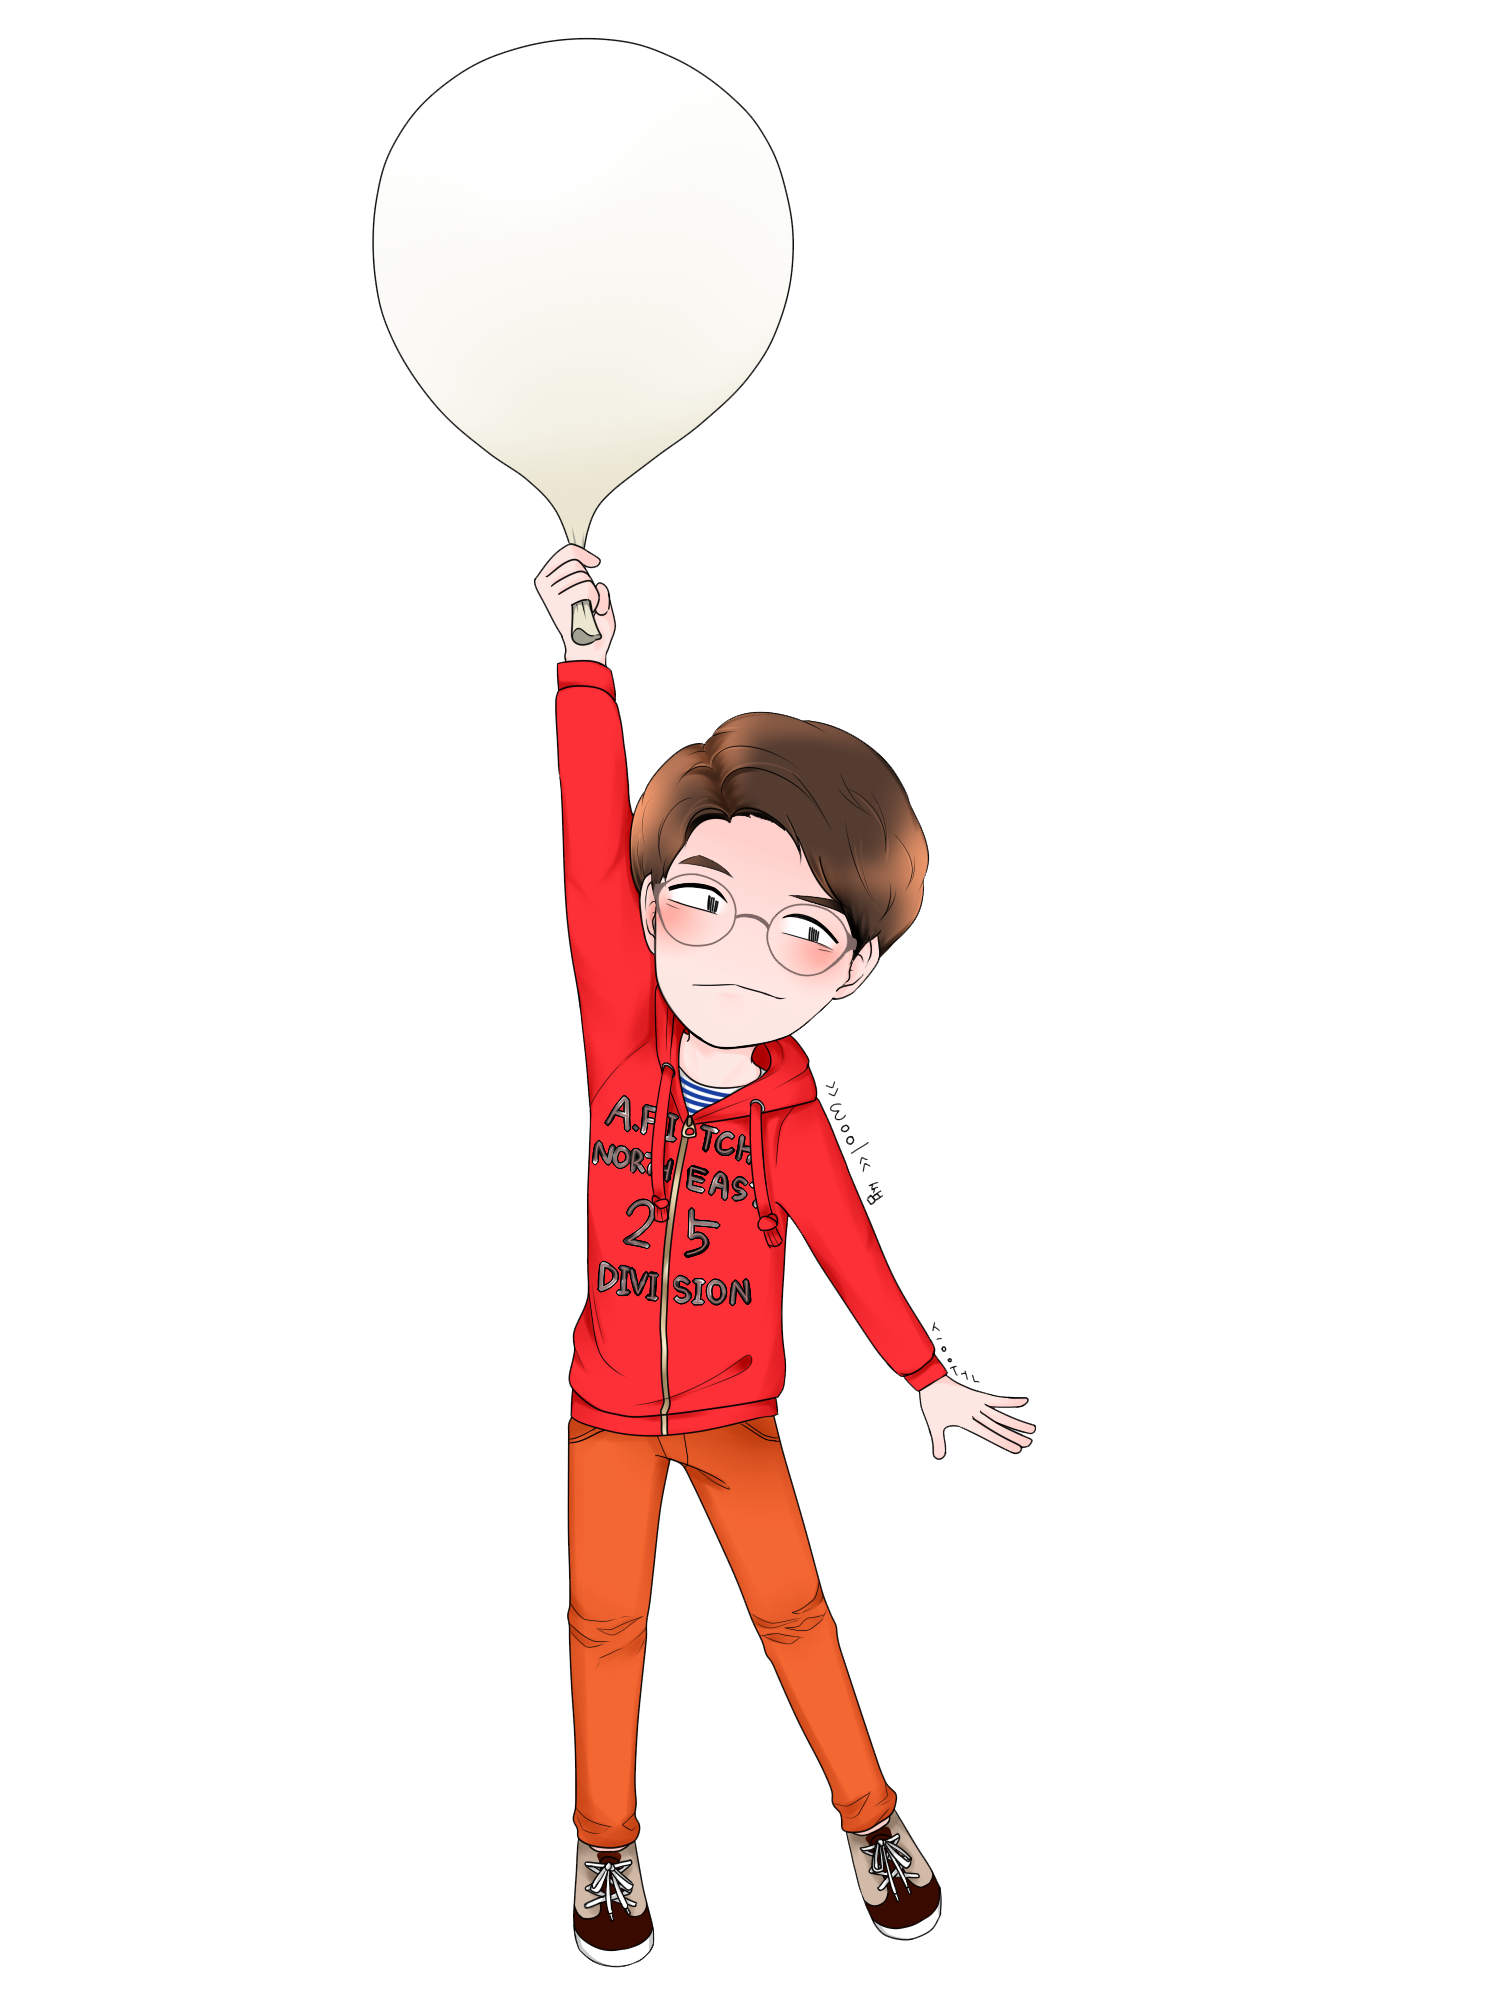
\includegraphics[width=0.4\paperwidth]{./logo/100_01.png}%
      
\includegraphics[width=0.7\paperwidth]{./logo/gshslogo2.jpg}%
    \end{picture}%
    }%
  \end{picture}%
  \vfill
  \vspace*{10mm}
  \raggedleft
  %% Title
  \usebeamerfont{title}\usebeamercolor[fg]{title}\inserttitle\par
  \vskip 2mm
  %% Subtitle
  \ifx\insertsubtitle\@empty
  \else\usebeamerfont{subtitle}\usebeamercolor[fg]{subtitle}\insertsubtitle
  \fi

  \vskip 3mm
  %% Horizontal line
  \usebeamercolor[fg]{title}\hrule height 2pt\hfill
  \vskip 10mm
  %% Author
  \usebeamercolor[fg]{author}\usebeamerfont{author}\insertauthor
  \vskip 1cm
  %% Institute
  \usebeamercolor[fg]{institute}\usebeamerfont{institute}\insertinstitute
  \vskip 1cm
  %% Date
  %\usebeamercolor[fg]{date}\usebeamerfont{date}\insertdate
  \vfill
}

%% itemize bullet setting %%
\setbeamertemplate{itemize items}[ball]

%% block setting %%
\setbeamertemplate{blocks}[rounded][shadow=true]

%% Title, Author, Institute, Date %%
\title[]{3D Print 사용 매뉴얼}
\subtitle[]{무한상상실}
\author[]{서울}
\institute[GSHS]{경기과학고등학교}
\date[]{\today}

%%%%%%%%%%%%%%%%%%%%%%%%%%%%%%%%%%%%%%%%%
%\logo{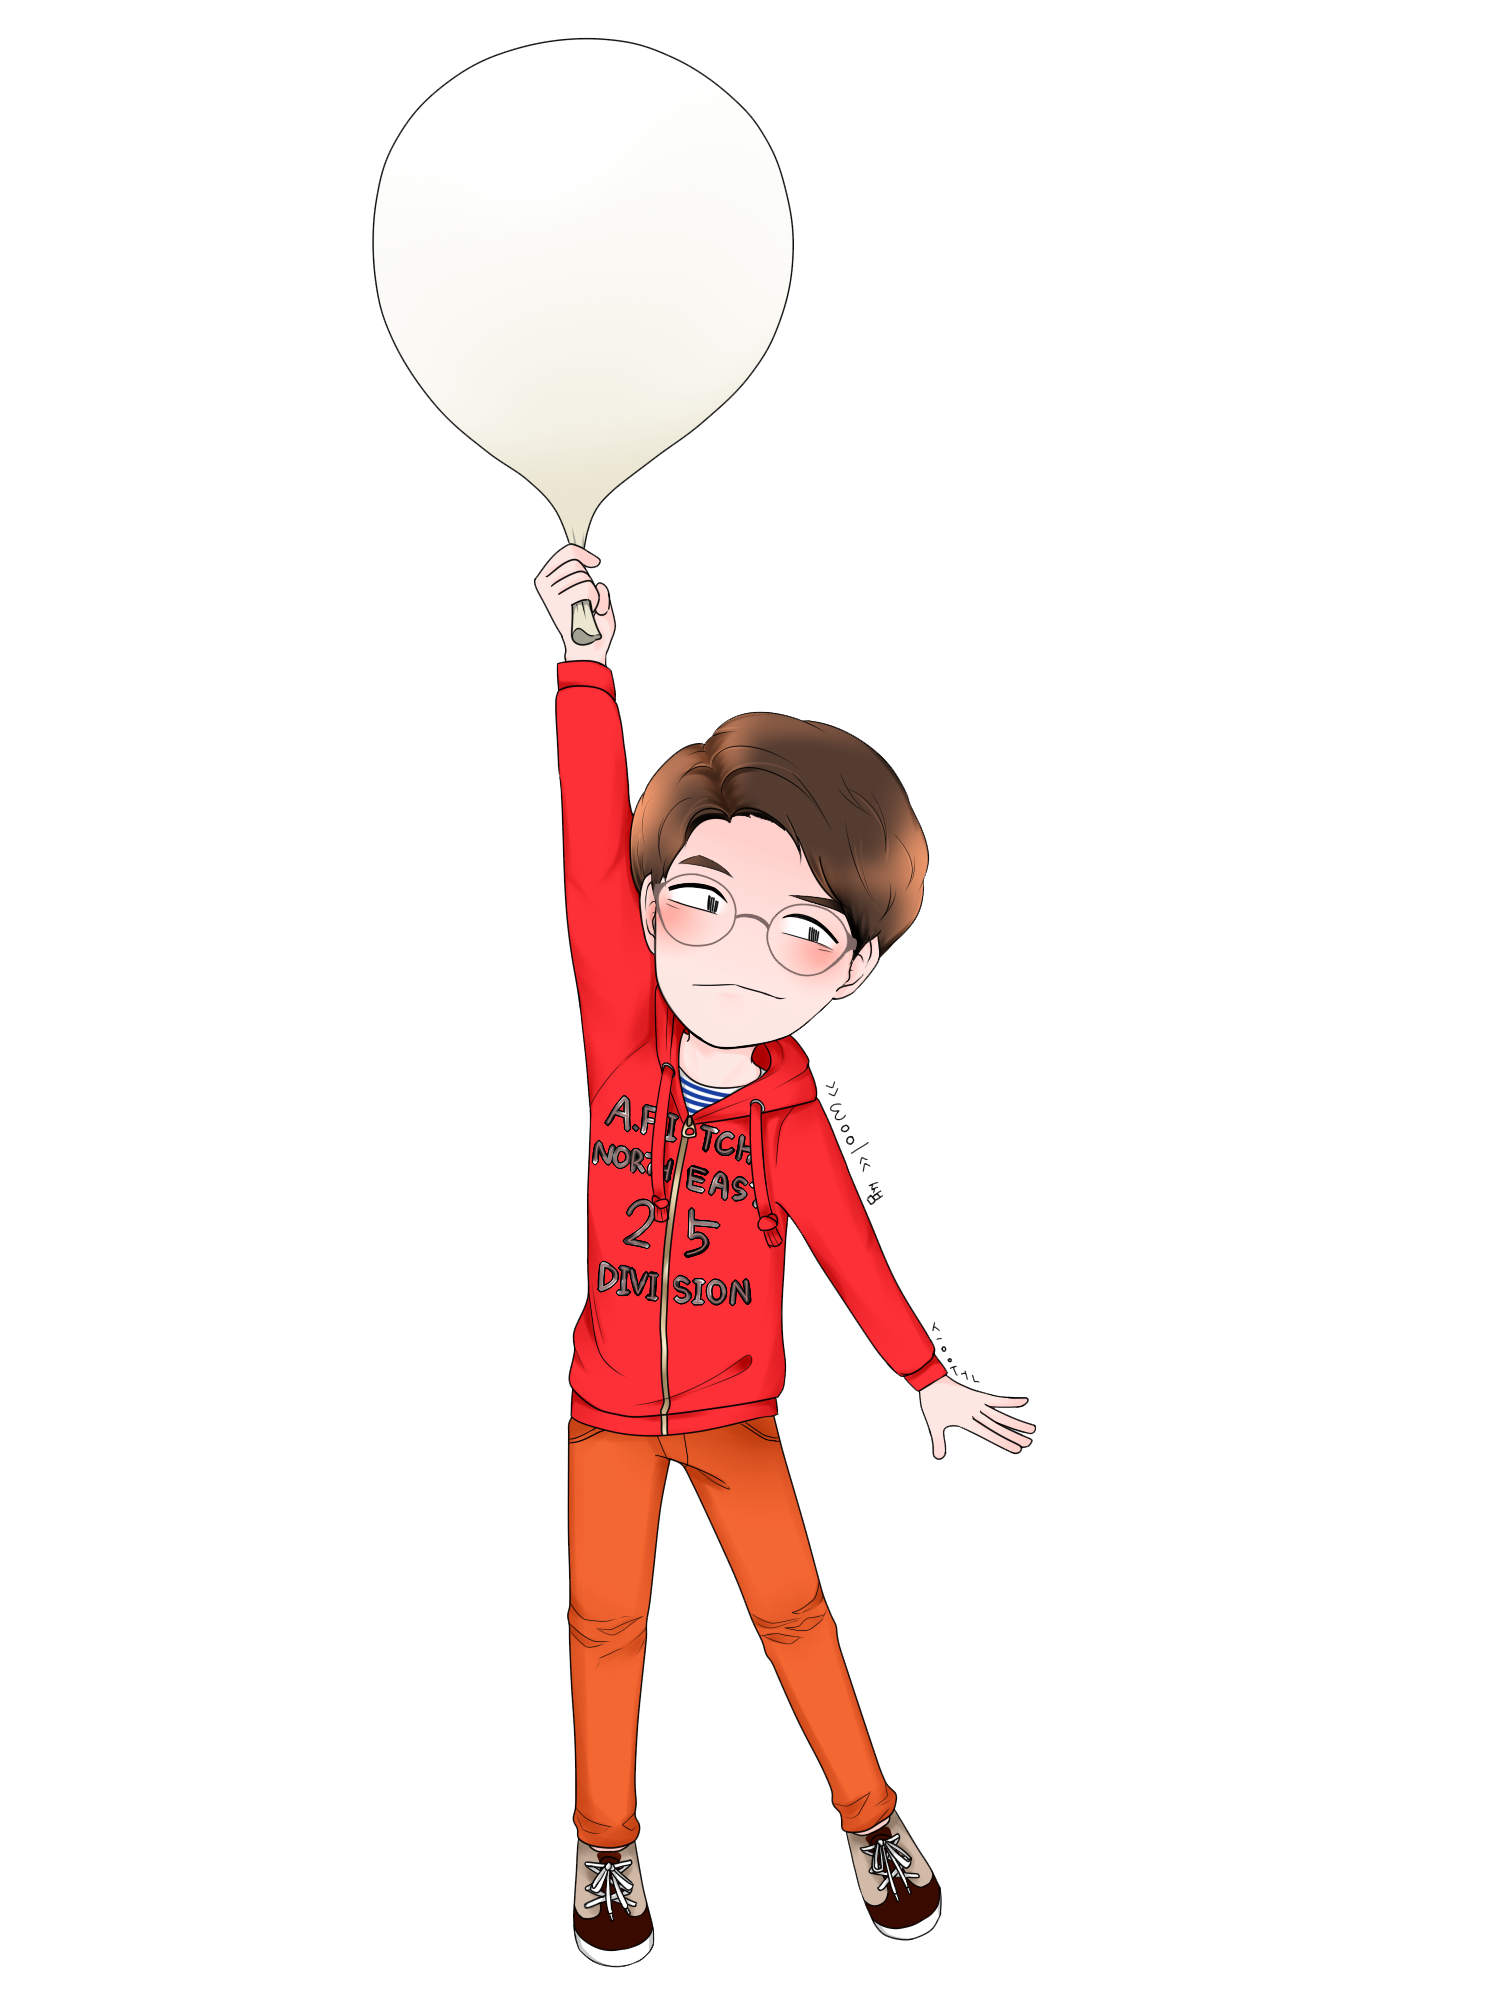
\includegraphics[width=15mm]{./logo/100_01.png}}
\logo{
\includegraphics[width=8mm]{./logo/gshslogo.png}}

%% Main %%
\begin{document}

\begin{frame}[plain]
\titlepage
\end{frame}
\setbeamertemplate{sidebar left}[sidebar theme]

\setstretch{1.3} %줄간격

\begin{comment}

\section{3D Printer}

\subsection{개요}

\begin{frame}[t]{역사}\footnotesize
\begin{itemize}
\item {\bf\large 1986년}
\begin{itemize}
\item  척 헐(Chuck Hull)
\item SLA방식 - 3D Systems. \\[15pt]
\end{itemize}
\item {\bf\large 1989년}
\begin{itemize}
\item 스콧 크럼프(Scott Crump)
\item FDM방식 - Stratasys. \\[15pt]
\end{itemize}
\item {\bf\large 2010년대}
\begin{itemize}
\item 3D프린터 특허가 풀리면서 대중화
\end{itemize}
\end{itemize}
\end{frame}


\begin{frame}[t]{개요}\footnotesize
\begin{itemize}
\item {\bf\large RP(Rapid Prototyping)}
\begin{itemize}
\item 디자인이나 기능성을 검토하기 위한 시제품 제작을 중심으로 한 개념 \\[15pt]
\end{itemize}
\item {\bf\large AM(Additive Manufacturing)}
\begin{itemize}
\item 최근에는 실제 사용 가능한 제품을 바로 제조하는 개념 \\[15pt]
\end{itemize}
\item {\bf\large 3D Printer}
\begin{itemize}
\item 대중적인 용어
\item 3D도면을 바탕으로 3차원 물체를 만들어내는 기계\cite{key1}
\end{itemize}
\end{itemize}
\end{frame}


\begin{frame}[t]{익스트루더(Extruder)와 베드(Bed)}\footnotesize
	\begin{center}
		%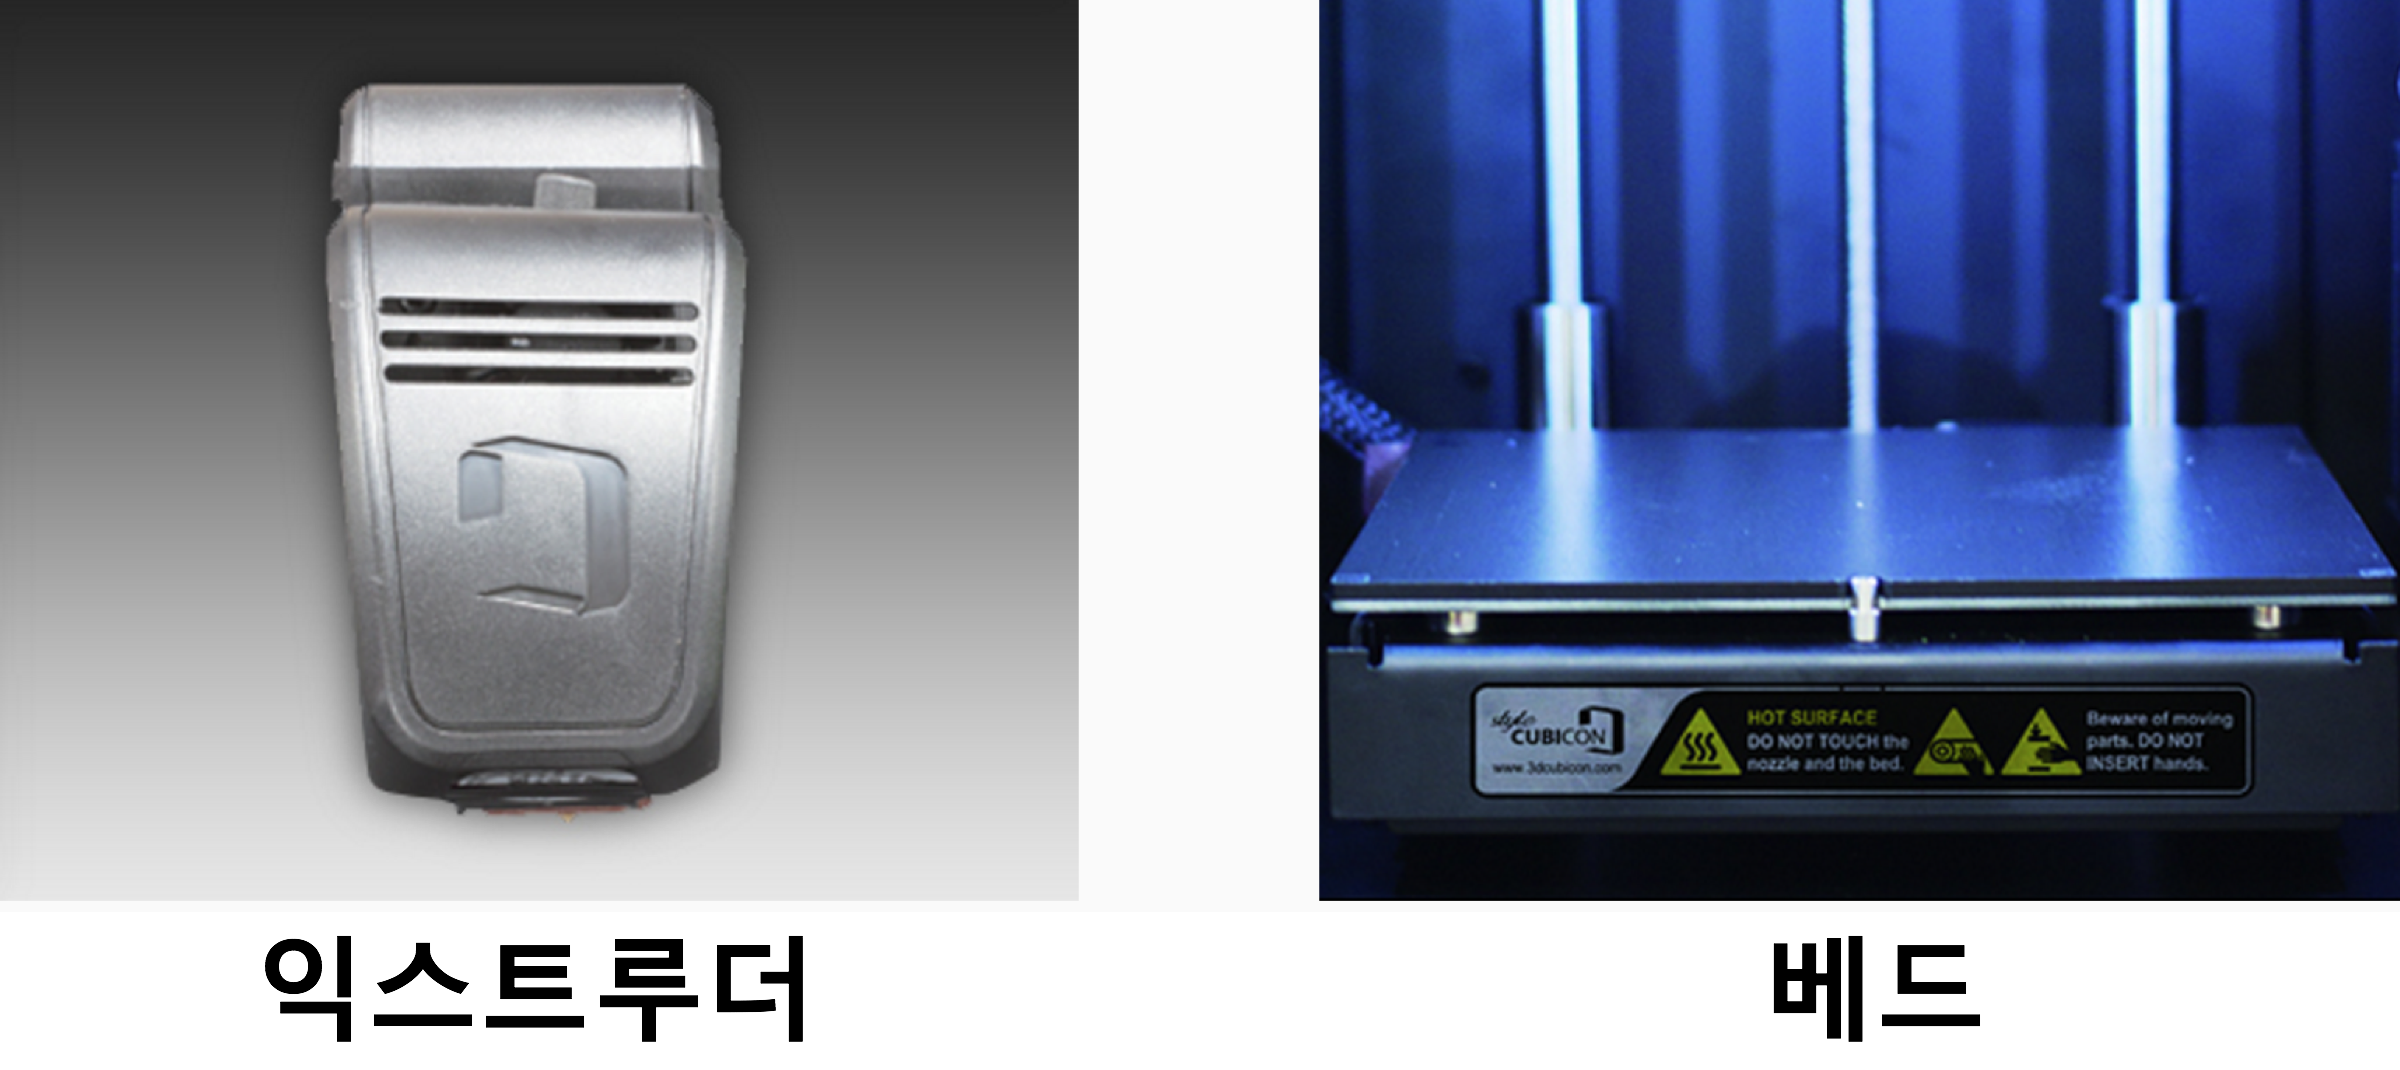
\includegraphics[width=9cm]{./image/18_09.png} %큐비콘
		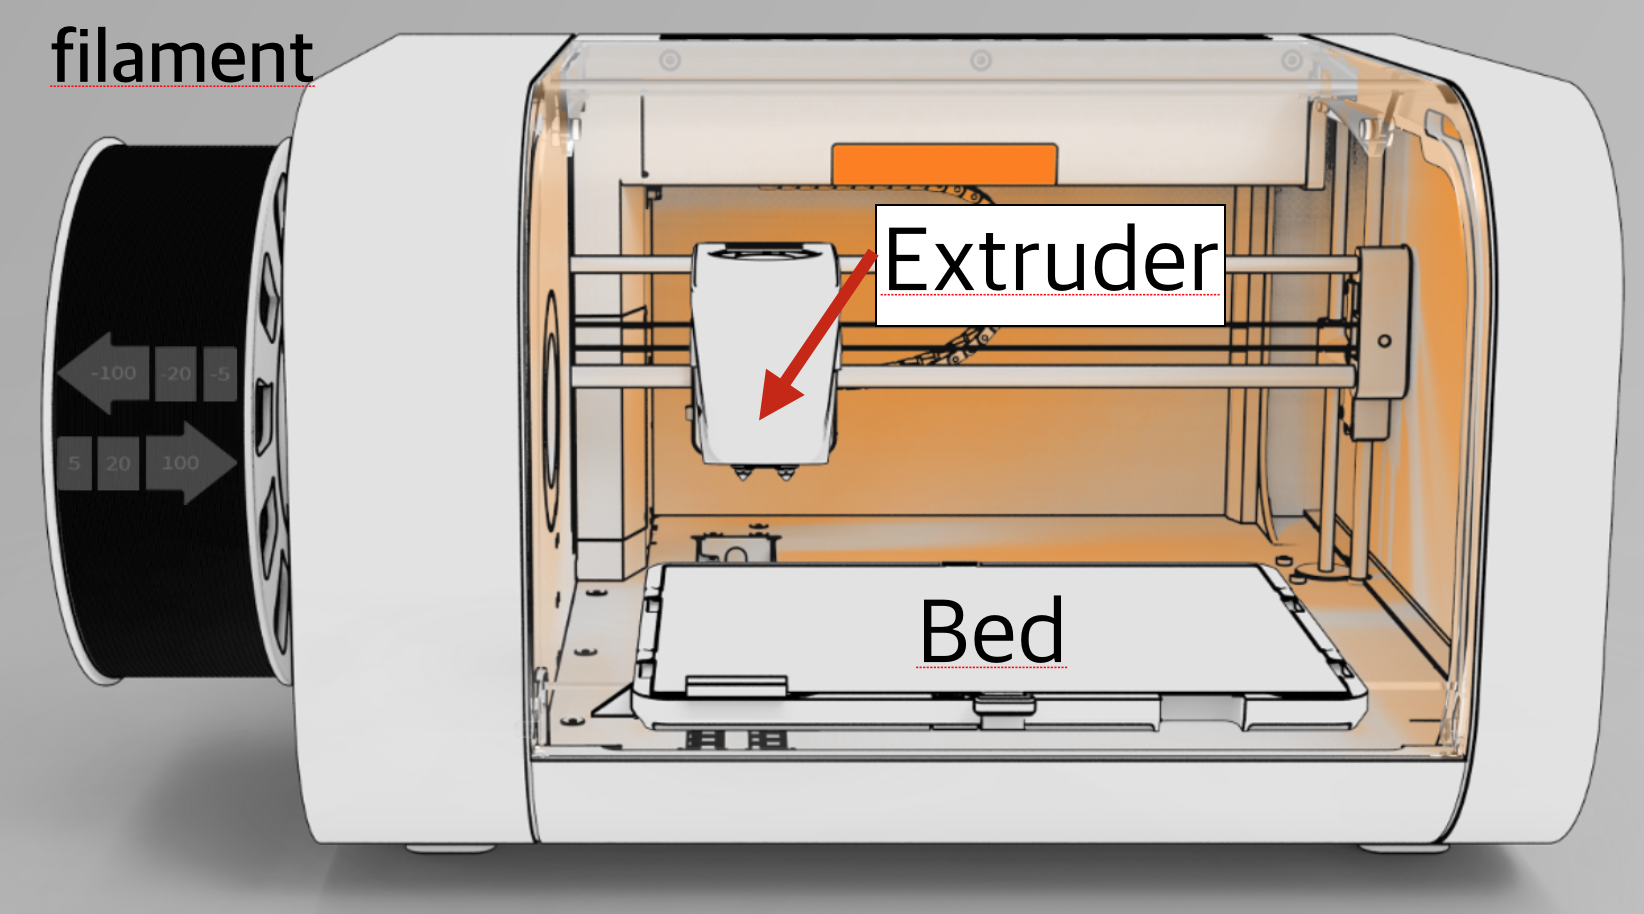
\includegraphics[height = 0.7\textheight]{./image/03_3dprinter.png} %robox
	\end{center}
\end{frame}

\subsection{종류/방식}

\begin{frame}[t]{FDM/FFF}\footnotesize
\begin{tabular}{lcr}
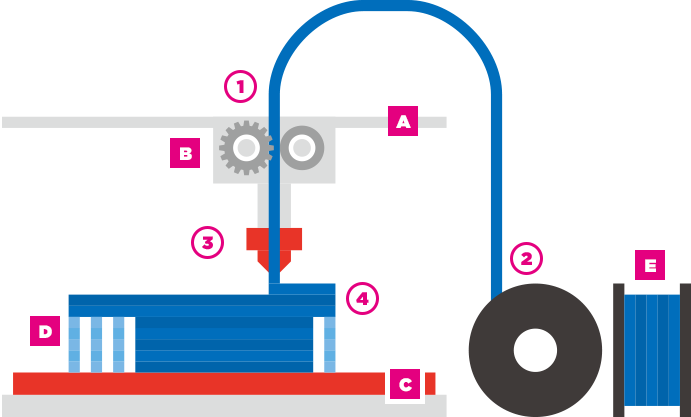
\includegraphics[width=0.8\textheight]{./image/04_1FFF.png}  &  & 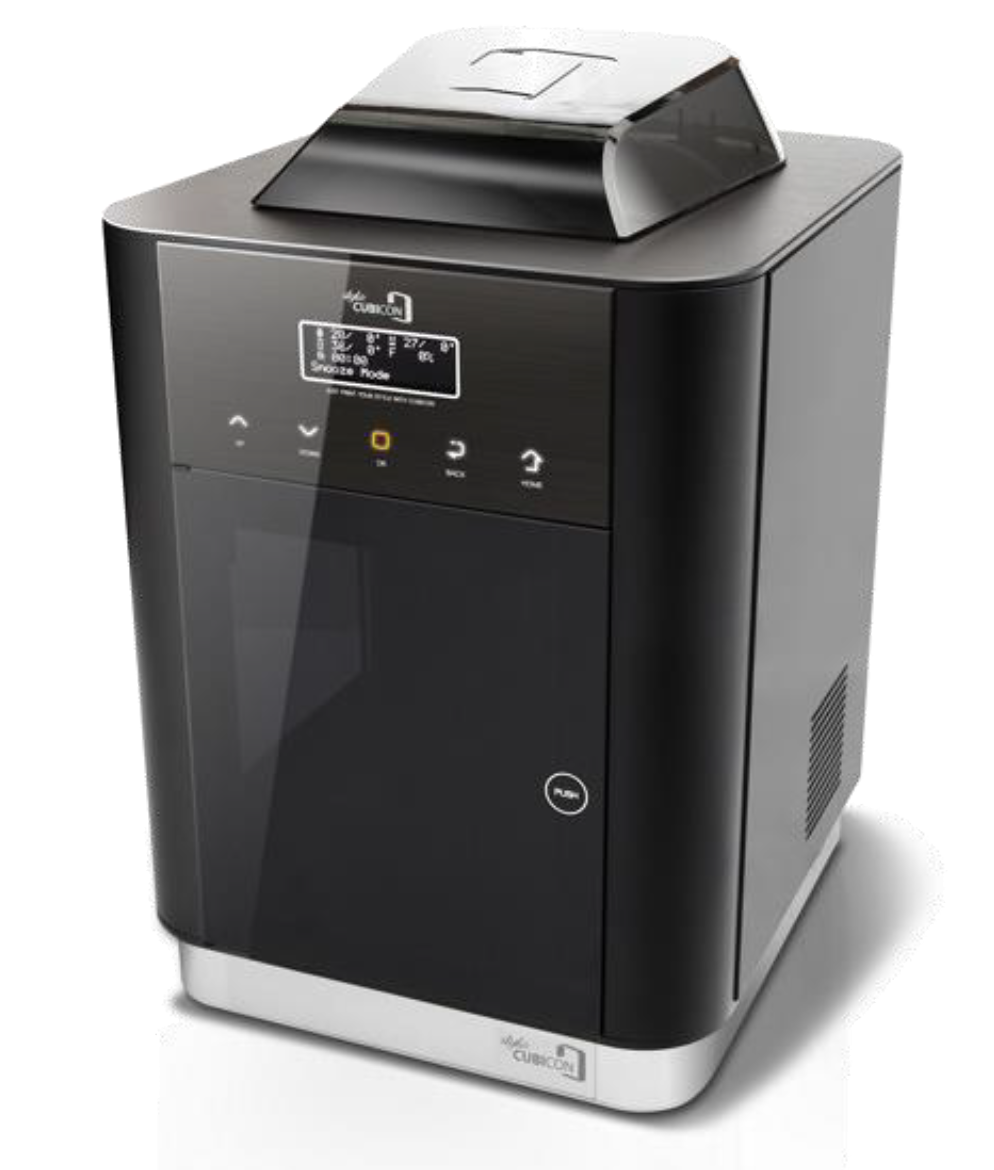
\includegraphics[width=0.4\textheight]{./image/18_01.png}
\end{tabular}
\begin{enumerate}[1.]
\item  익스트루더가 원료 필라멘트를 끌어당깁니다. 
\item  필라멘트 스풀의 필라멘트가 당겨집니다.
\item 고체 필라멘트를 녹일 수 있는 온도로 달궈진 핫-엔드 노즐에서 원료를 압출합니다.
\item 압출된 원료는 설정된 값만큼 한 층씩 적층되며 조형합니다.
\end{enumerate}
\end{frame}

\begin{frame}[t]{FDM/FFF}\footnotesize
%\movie[width = 1.0\textwidth, showcontrols]{./image/04_fff_printing.mp4}
\end{frame}

\begin{frame}[t]{SLA}\footnotesize
\begin{tabular}{lcr}
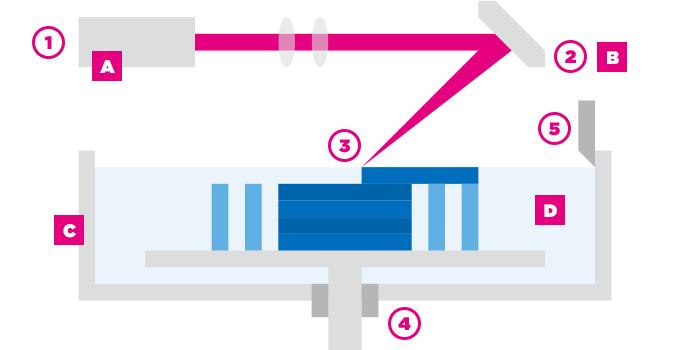
\includegraphics[width=0.8\textheight]{./image/05_1SLA.png}  &  & 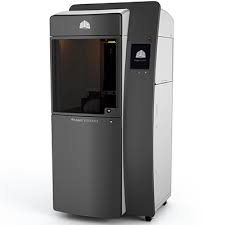
\includegraphics[width=0.4\textheight]{./image/05_2SLA.jpeg}
\end{tabular}
\begin{enumerate}[1.]
\item 레이저를 조사합니다.
\item 다이내믹 미러가 X,Y 축으로 움직이며 전달받은 레이저 빔을 수조에 정확히 전달합니다.
\item 수조 안에 있던 광경화 수지가 레이저 빔에 의해 굳어집니다.
\item 수조 안에 있는 조형판은 한 층씩 수지가 굳어질 때마다 정해진 층의 두께만큼 내려갑니다.
 \item 리코터 블레이드가 인쇄물의 표면을 지나가며 평탄화 작업을 합니다.
\end{enumerate}
\end{frame}

\begin{frame}[t]{DLP}\footnotesize
\begin{tabular}{lcr}
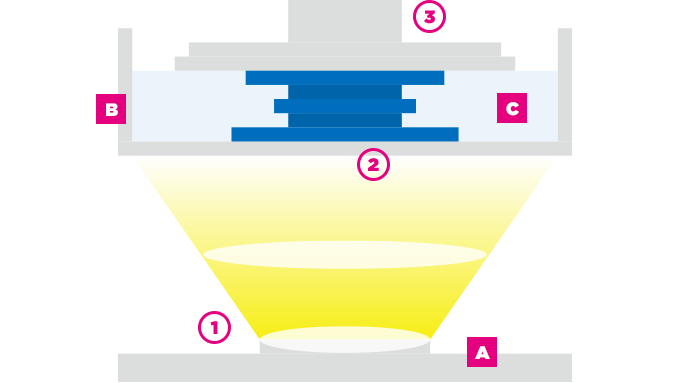
\includegraphics[width=0.8\textheight]{./image/06_1DLP.png}  &  & 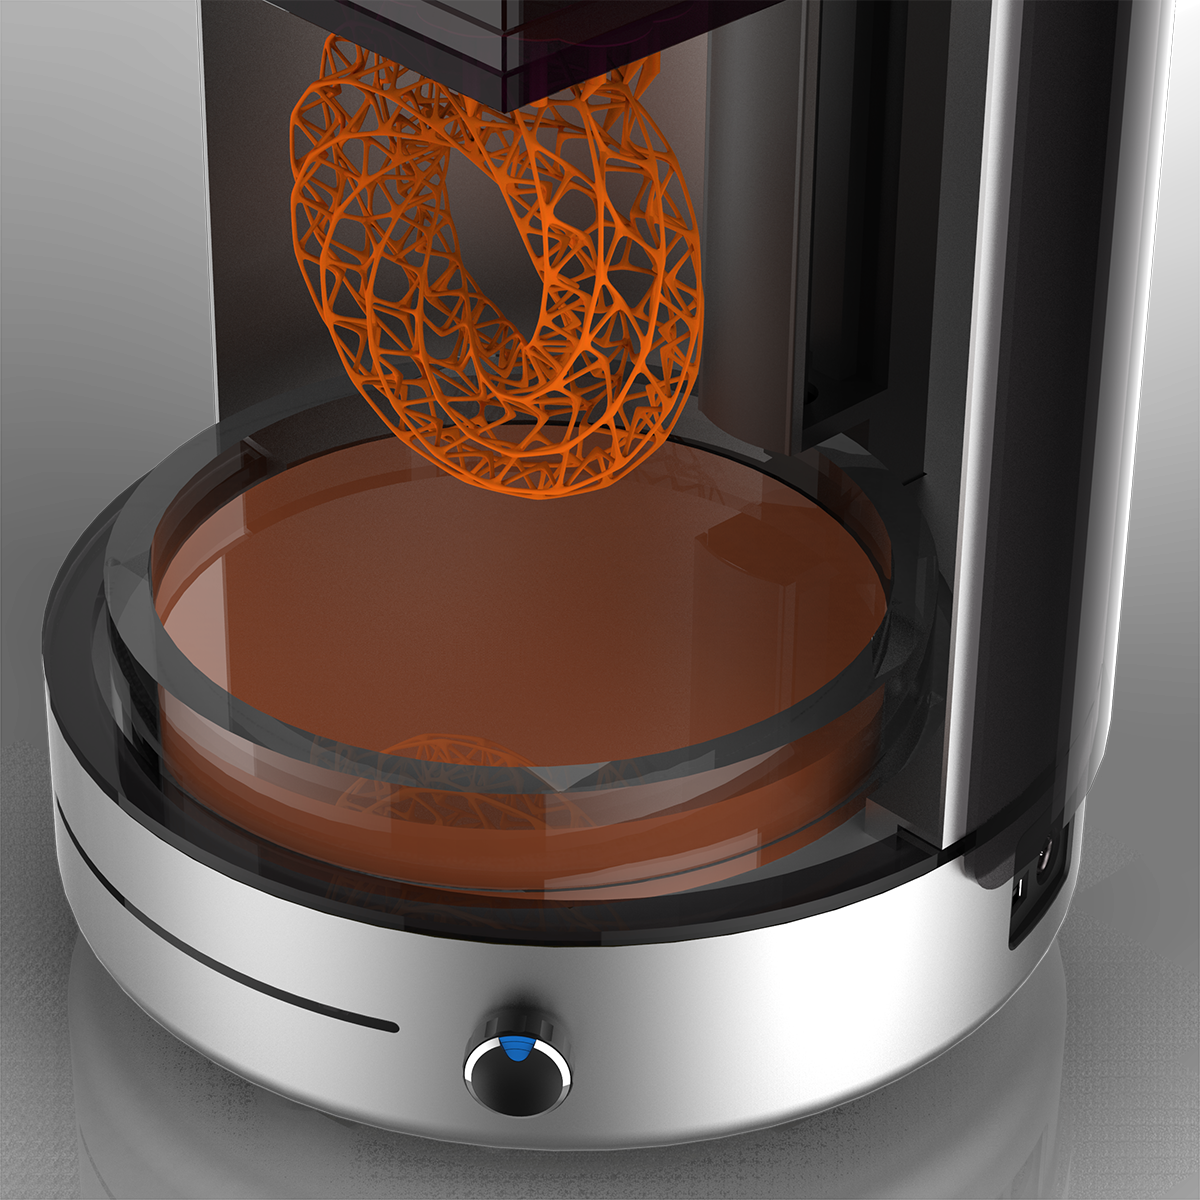
\includegraphics[width=0.4\textheight]{./image/06_2DLP.png}
\end{tabular}
\begin{enumerate}[1.]
\item DLP 프로젝터가 조형 이미지를 조사합니다.
\item 수조 안에 있던 광경화 수지가 디지털 라이트에 의해 굳어집니다.
\item 수조 안에 있는 조형판은 한 층씩 수지가 굳어질 때마다 정해진 층의 두께만큼 올라갑니다.
\end{enumerate}
\end{frame}

\begin{frame}[t]{OLO}\footnotesize
\begin{center}
%\movie{./image/04_fff_printing.mp4}
\end{center}
\end{frame}

\subsection{현재와 미래}

\begin{frame}[t]{3D프린터의 현재}\footnotesize
\begin{tabular}{lcr}
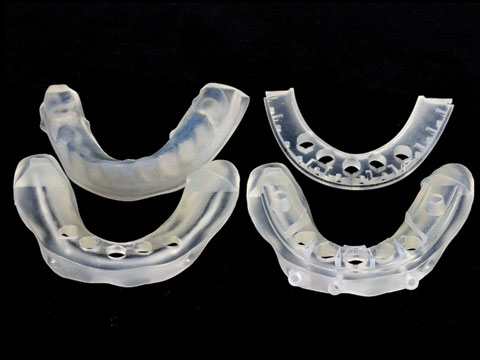
\includegraphics[width=0.6\textheight]{./image/07_1.jpg}  & 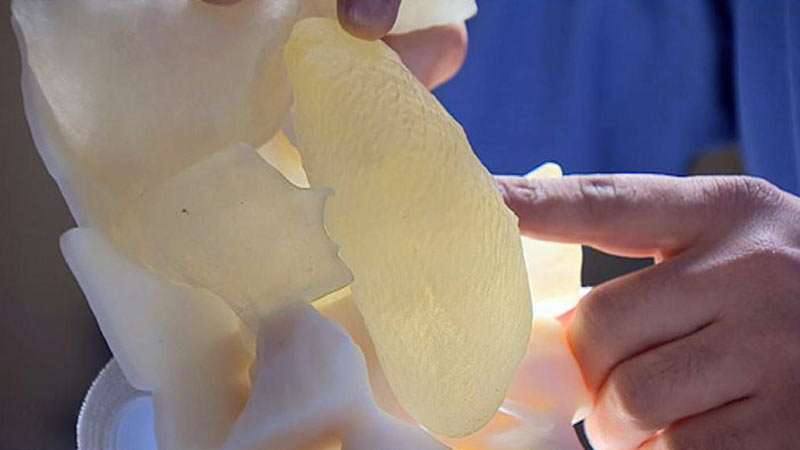
\includegraphics[width=0.6\textheight]{./image/07_2.jpg} \\
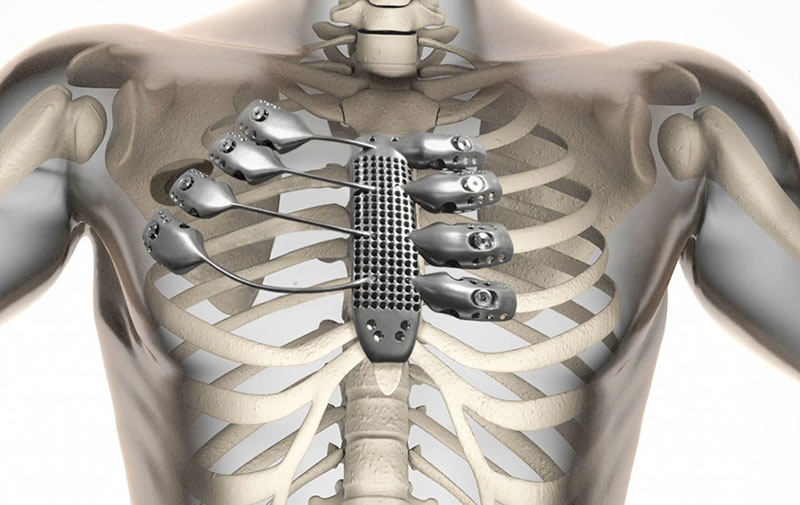
\includegraphics[width=0.6\textheight]{./image/07_3.jpg}  & 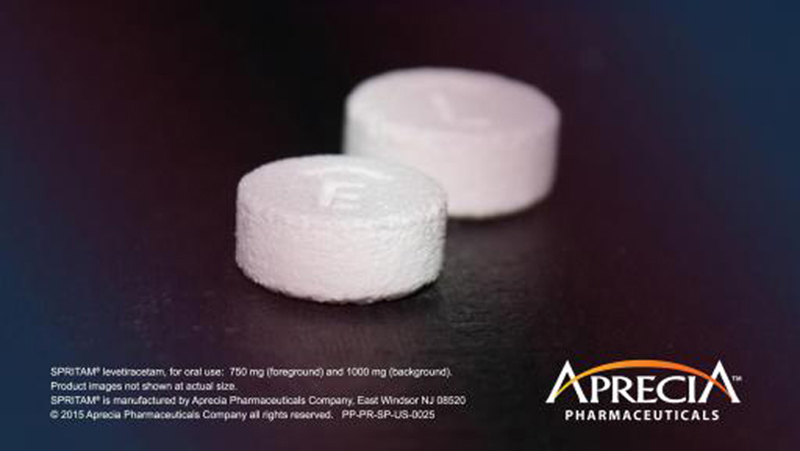
\includegraphics[width=0.6\textheight]{./image/07_4.jpg} 
\end{tabular}
\end{frame}

\begin{frame}[t]{3D프린터의 현재}\footnotesize
\begin{tabular}{lcr}
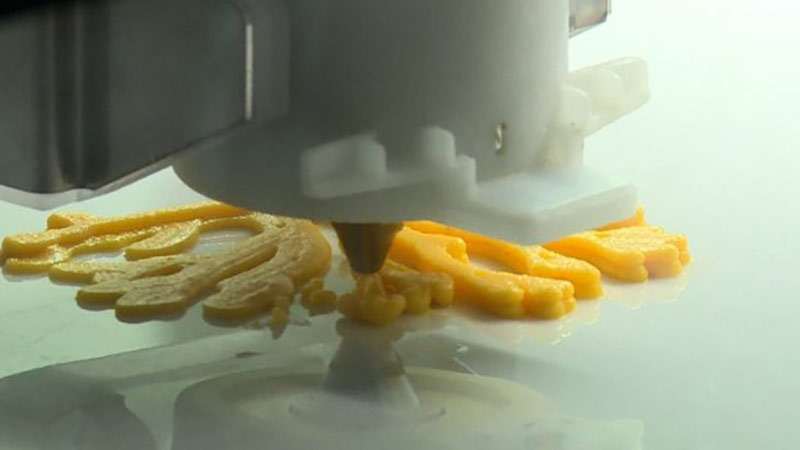
\includegraphics[width=0.6\textheight]{./image/07_5.jpg}  & 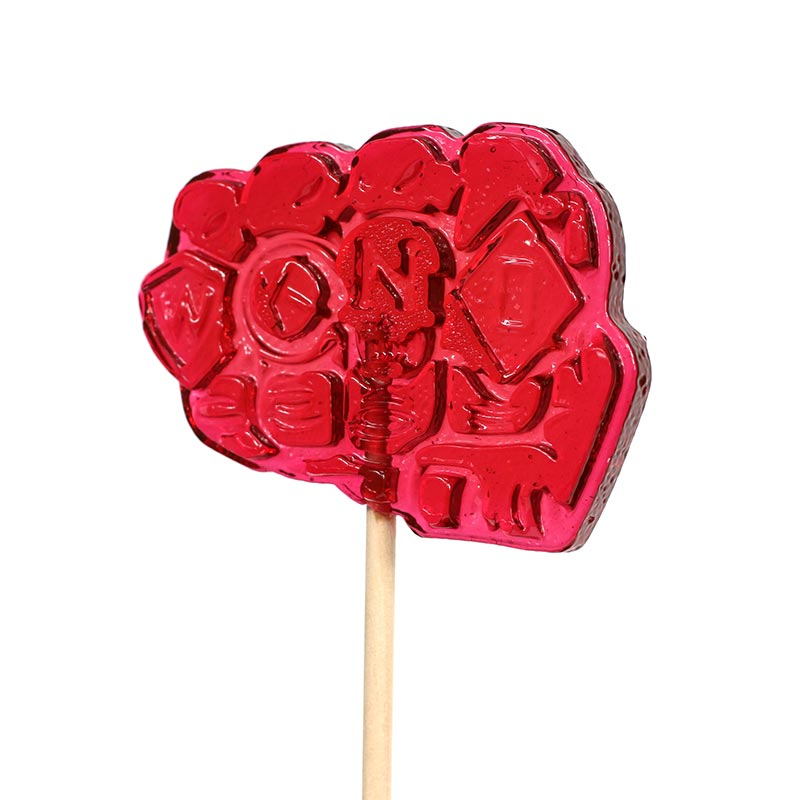
\includegraphics[width=0.4\textheight]{./image/07_6.jpg} \\
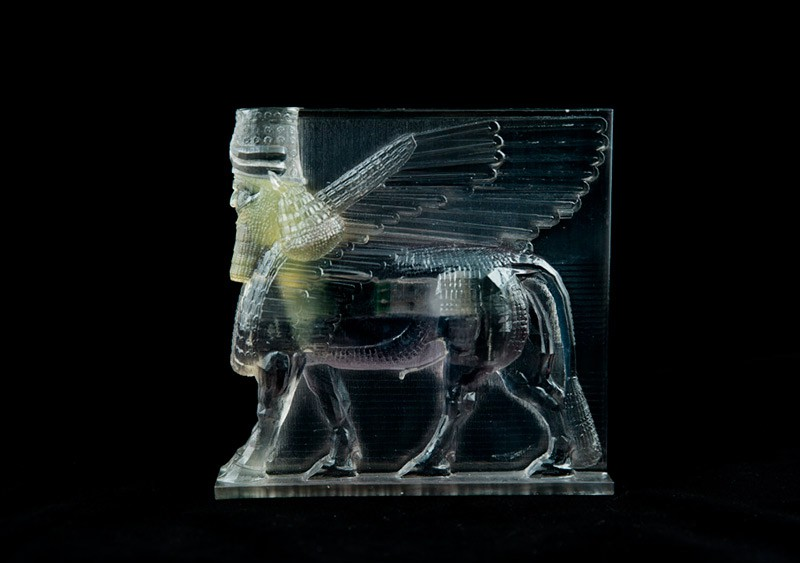
\includegraphics[width=0.6\textheight]{./image/07_7.jpg}  & 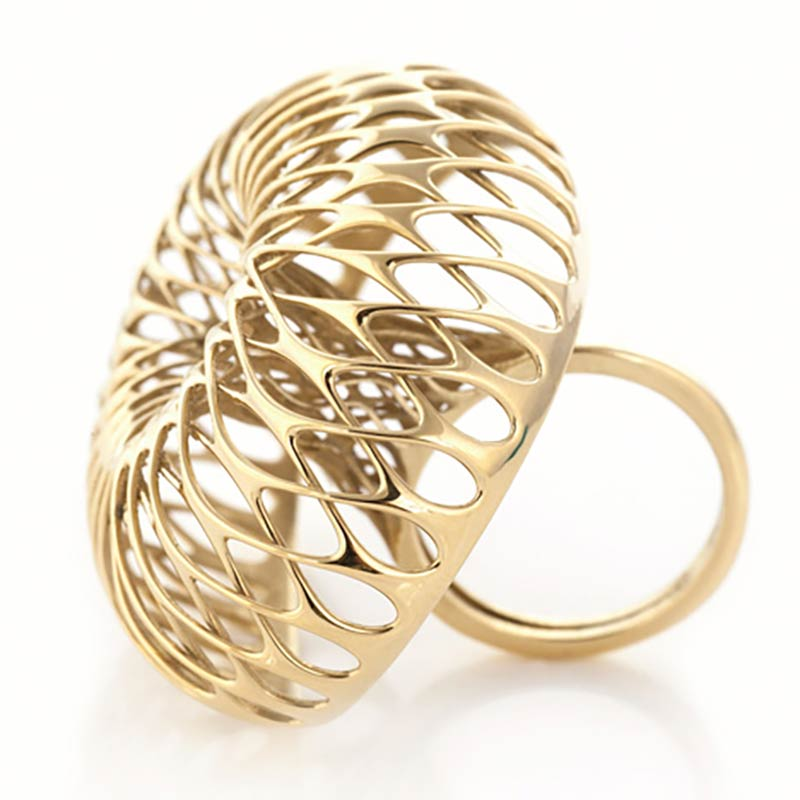
\includegraphics[width=0.4\textheight]{./image/07_8.jpg} 
\end{tabular}
\end{frame}

\begin{frame}[t]{3D프린터의 현재}\footnotesize
\begin{tabular}{lcr}
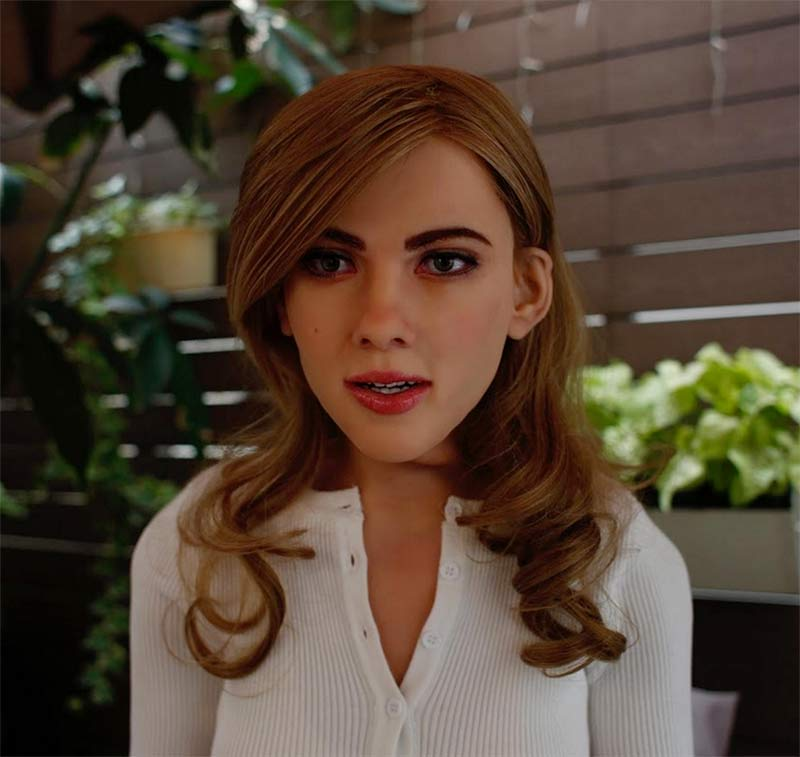
\includegraphics[width=0.4\textheight]{./image/07_9.jpg}  & 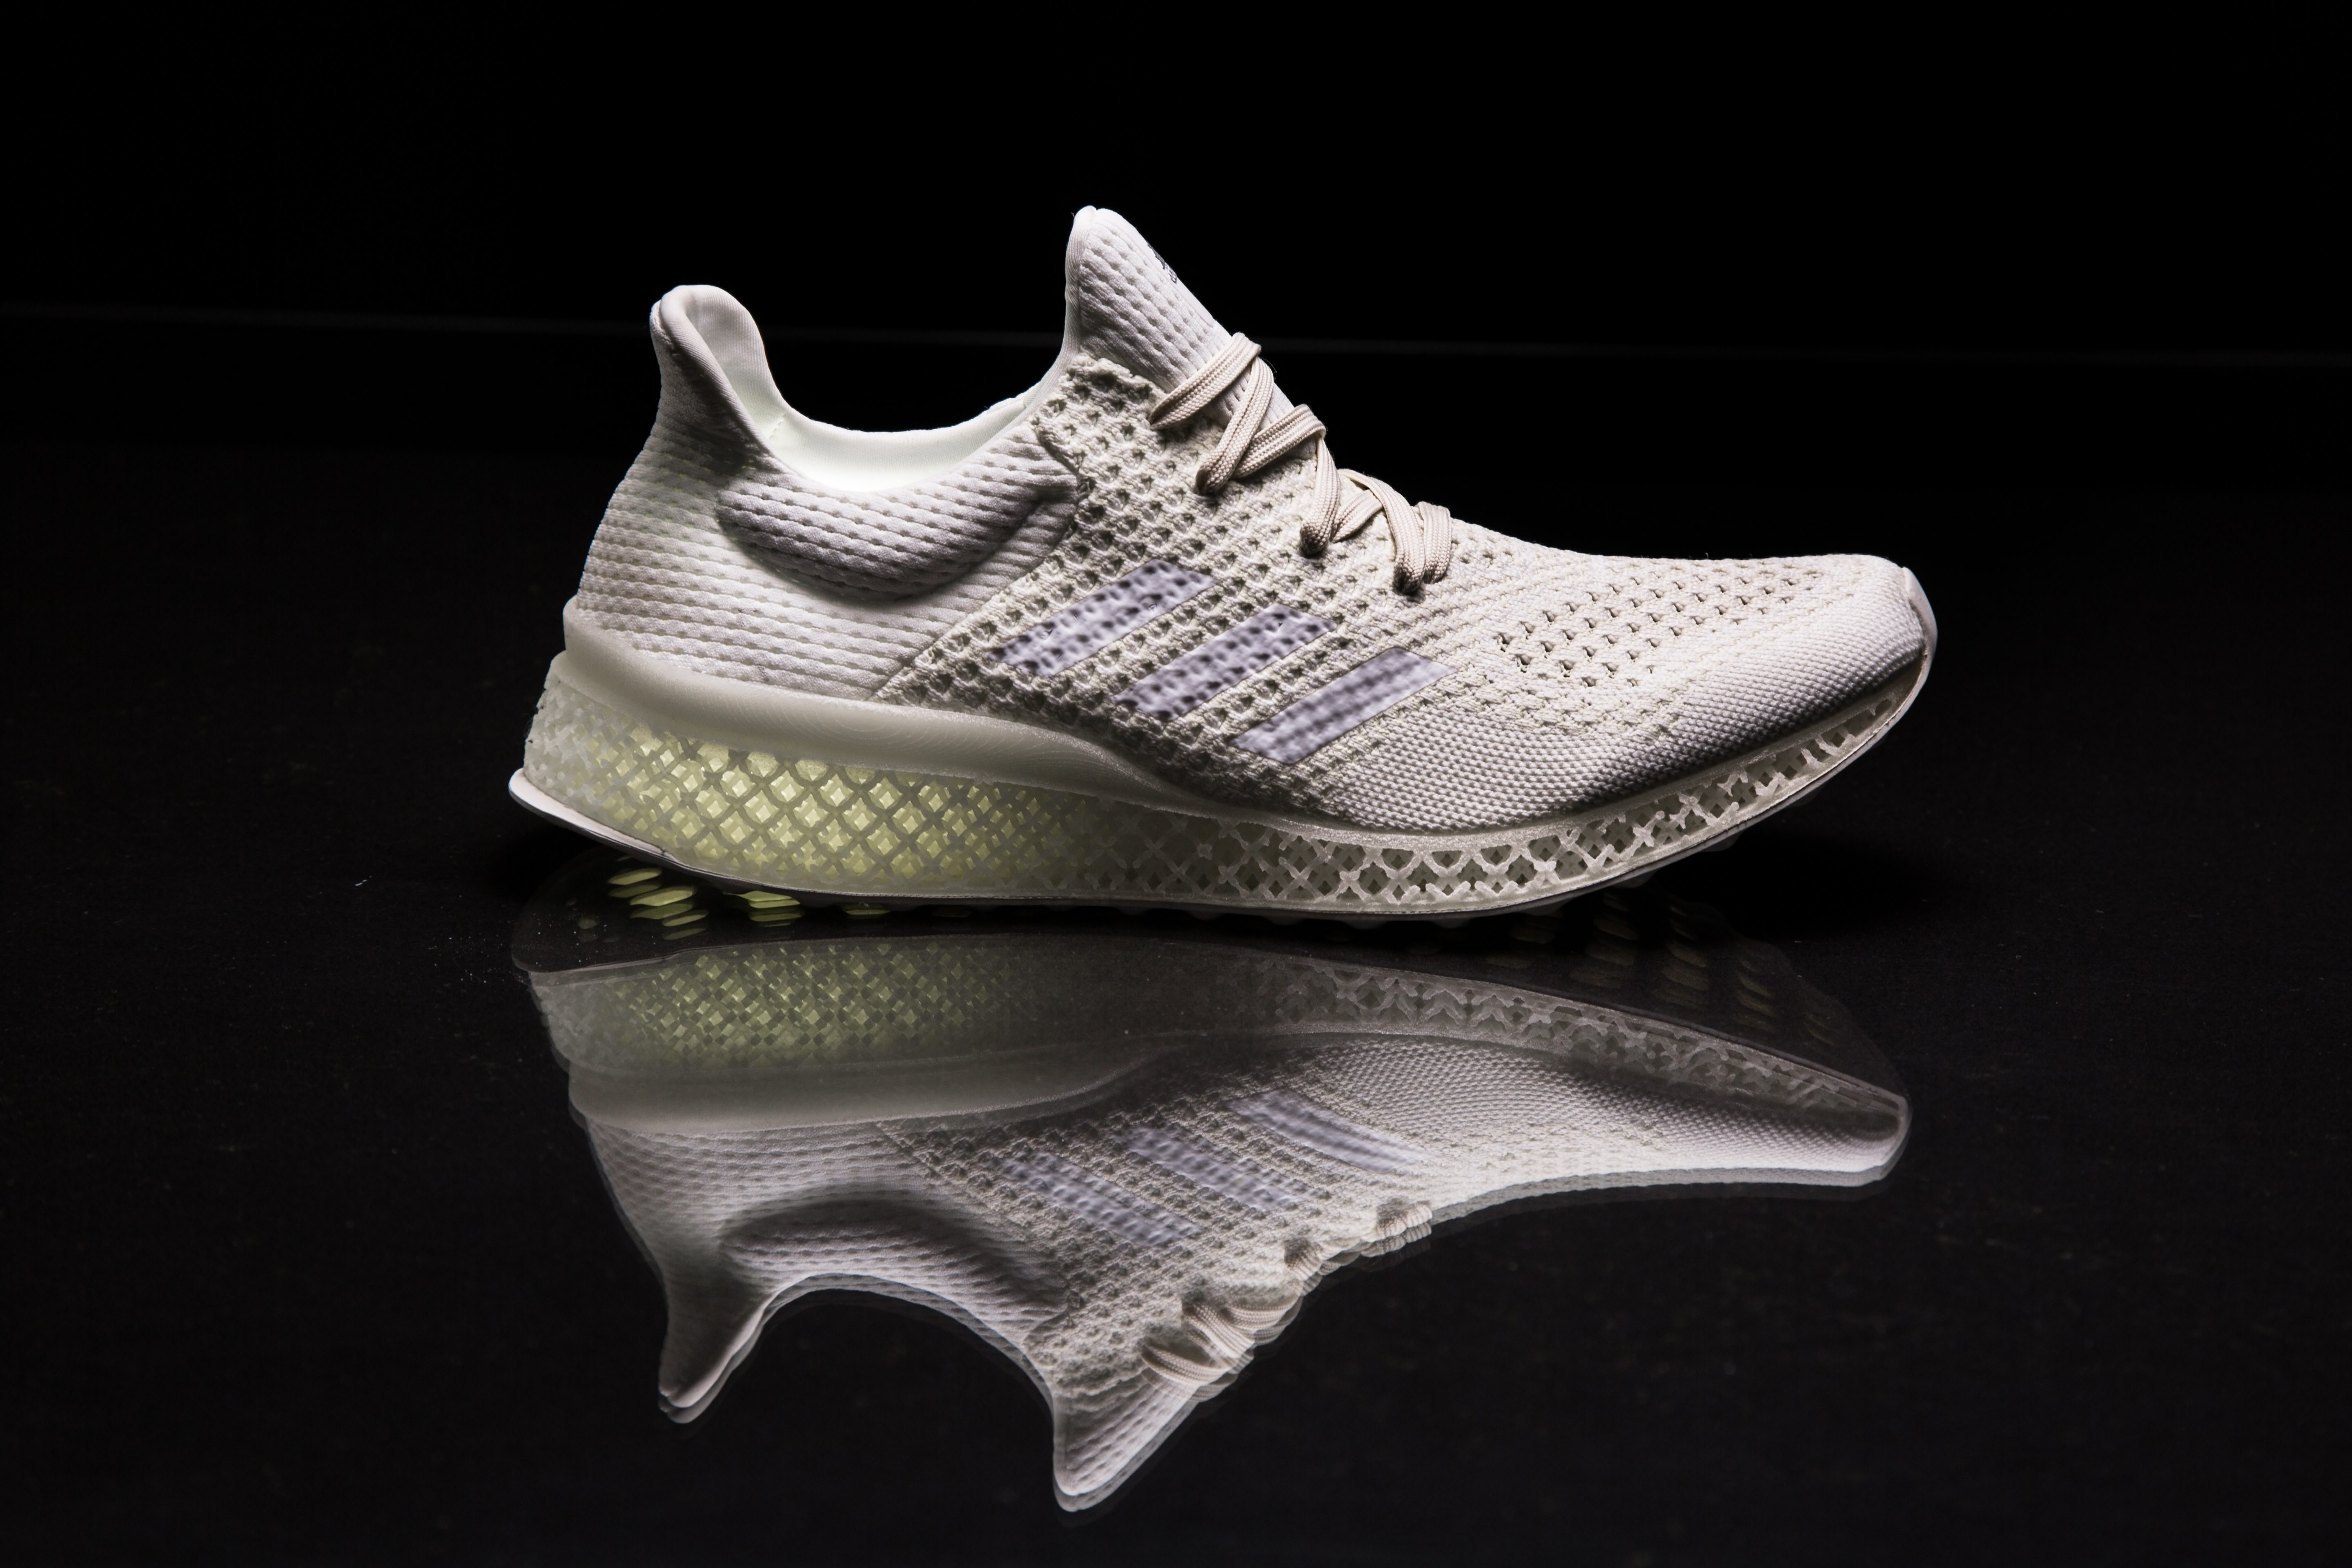
\includegraphics[width=0.6\textheight]{./image/07_10.jpg} \\
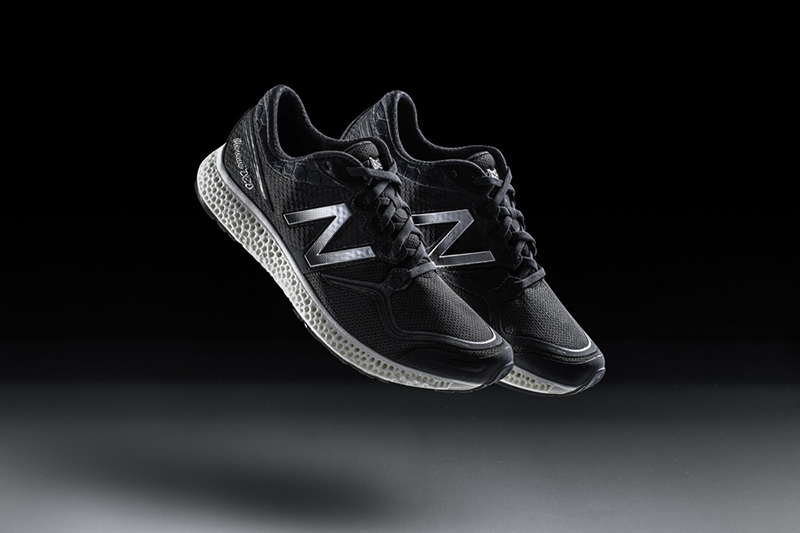
\includegraphics[width=0.6\textheight]{./image/07_11.jpg}  & 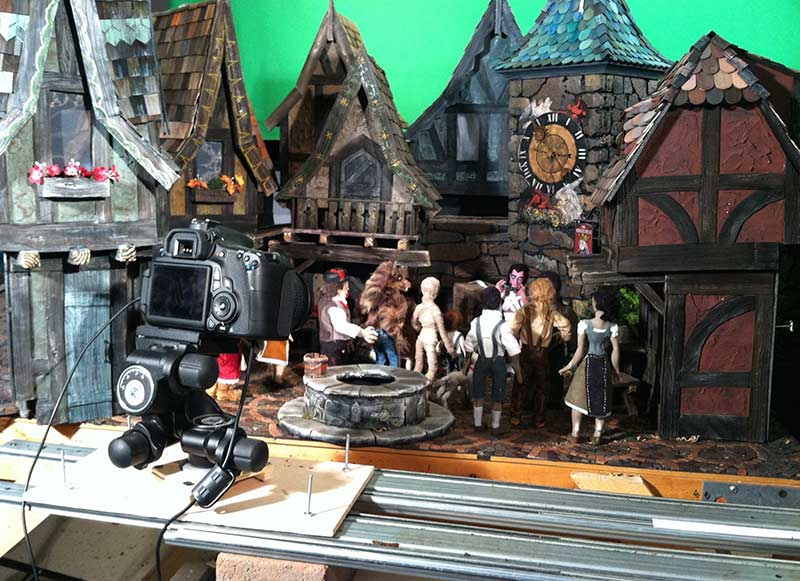
\includegraphics[width=0.6\textheight]{./image/07_12.jpg} 
\end{tabular}
\end{frame}

\begin{frame}[t]{3D프린터의 현재}\footnotesize
\begin{tabular}{lcr}
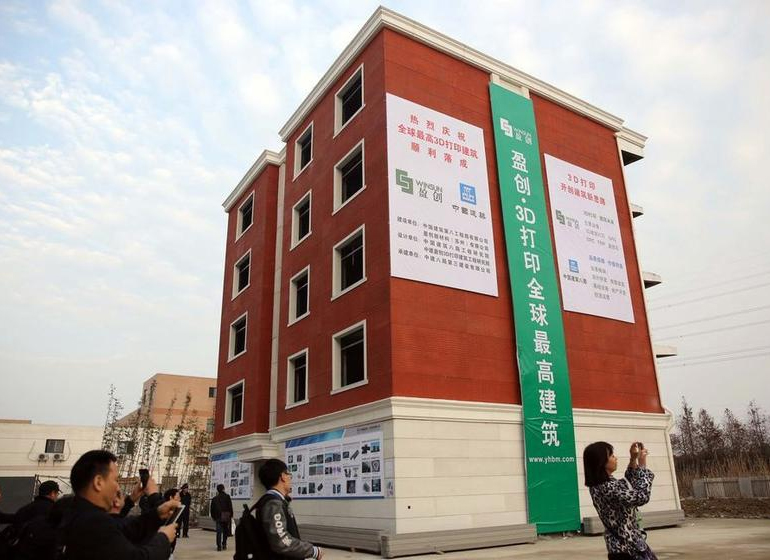
\includegraphics[width=0.5\textheight]{./image/07_13.jpg}  & 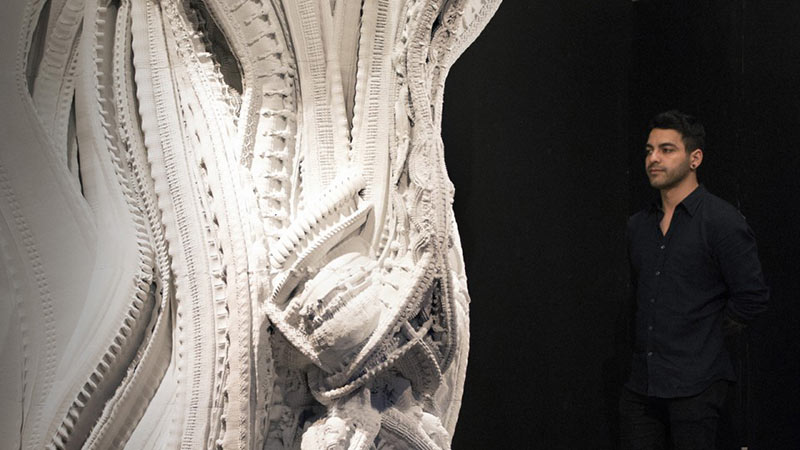
\includegraphics[width=0.6\textheight]{./image/07_14.jpg} \\
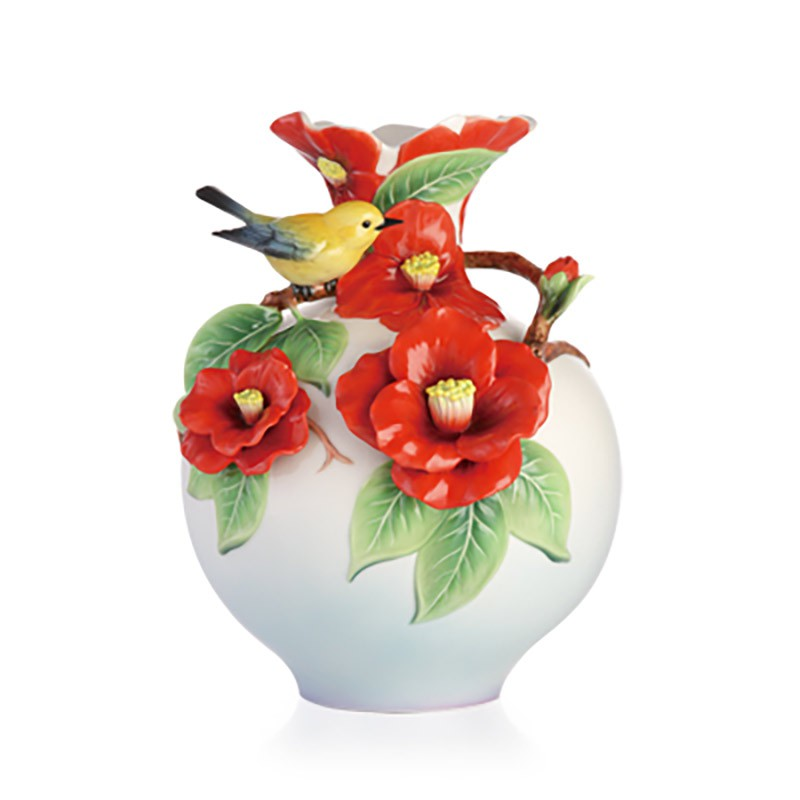
\includegraphics[width=0.5\textheight]{./image/07_15.jpg}  & 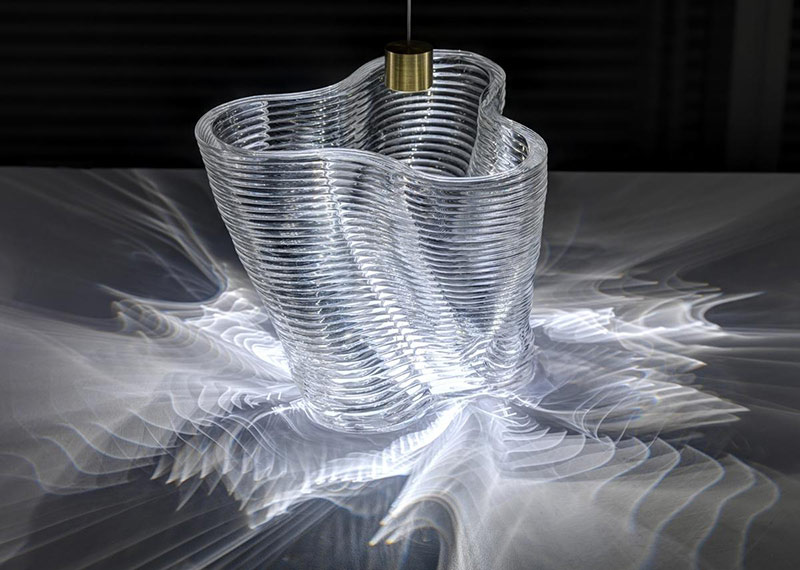
\includegraphics[width=0.6\textheight]{./image/07_16.jpg} 
\end{tabular}
\end{frame}

\begin{frame}[t]{3D프린터의 현재}\footnotesize
\begin{tabular}{lll}
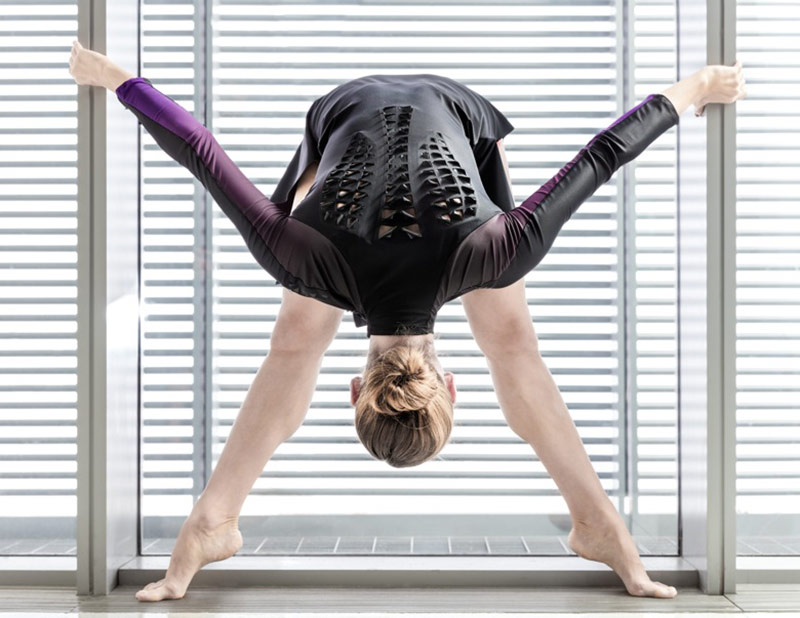
\includegraphics[width=0.5\textheight]{./image/07_20.jpg}&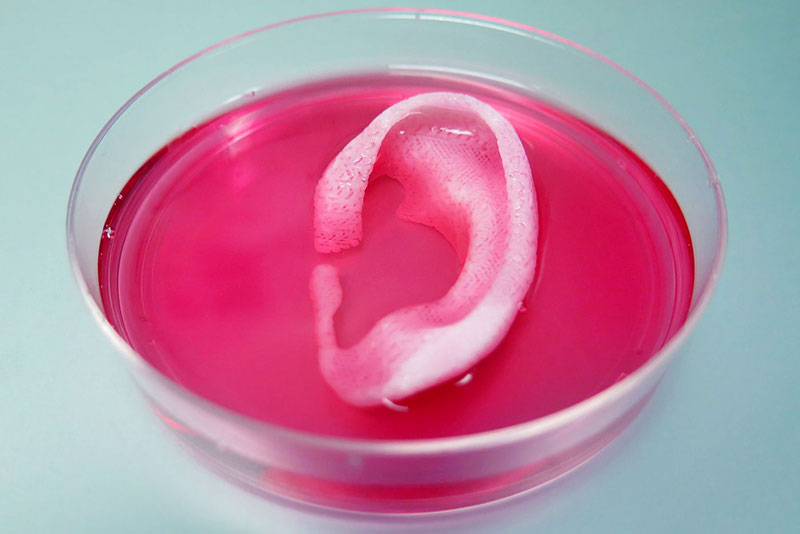
\includegraphics[width=0.5\textheight]{./image/07_21.jpg} \\
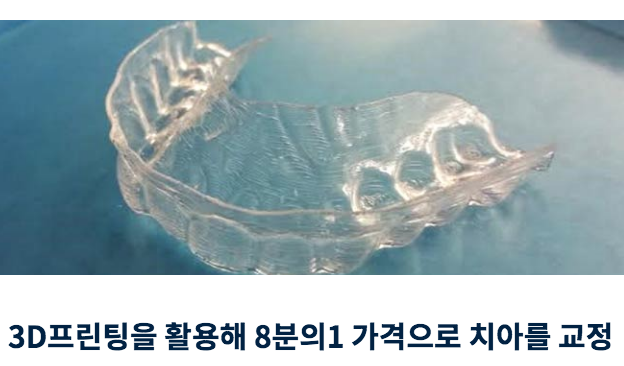
\includegraphics[width=0.8\textheight]{./image/07_17.png}
\end{tabular}
\end{frame}

\begin{frame}[t]{3D프린터의 현재}\footnotesize
\begin{tabular}{lcr}
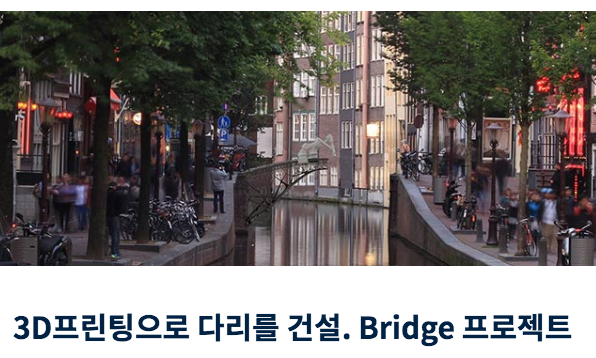
\includegraphics[width=0.7\textheight]{./image/07_18.png} \\
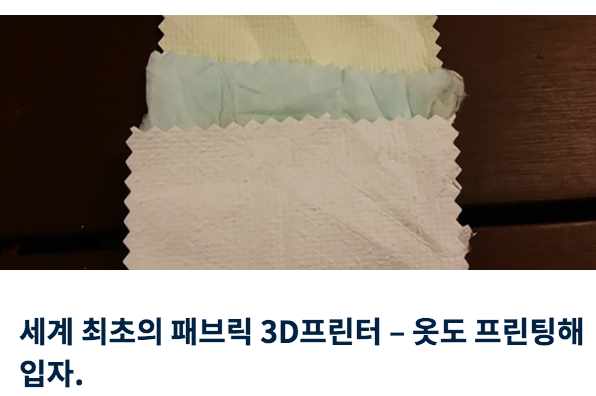
\includegraphics[width=0.7\textheight]{./image/07_19.png}
\end{tabular}
\end{frame}

\begin{frame}[t]{3D프린터의 미래}\footnotesize
\begin{tabular}{lcr}
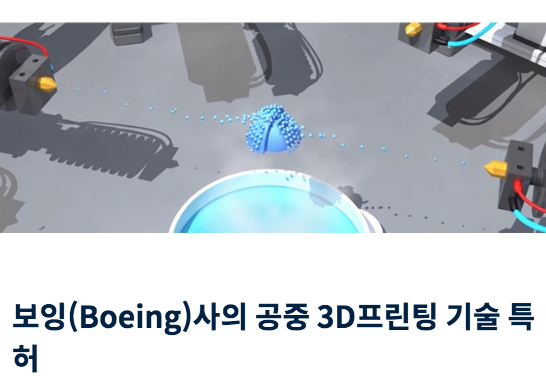
\includegraphics[width=0.7\textheight]{./image/08_01.png} \\
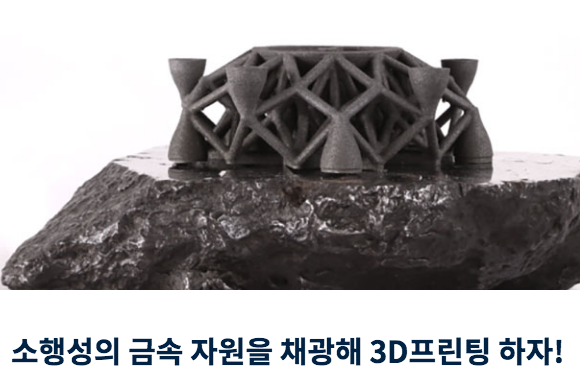
\includegraphics[width=0.7\textheight]{./image/08_02.png}
\end{tabular}
\end{frame}

\begin{frame}[t]{3D프린터의 미래}\footnotesize
\begin{tabular}{lcr}
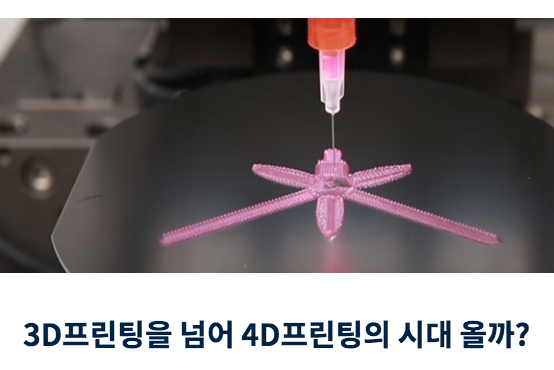
\includegraphics[width=0.7\textheight]{./image/08_03.png} \\
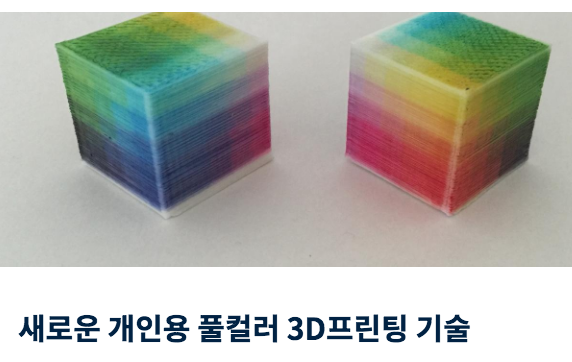
\includegraphics[width=0.7\textheight]{./image/08_04.png}
\end{tabular}
\end{frame}

\begin{frame}[t]{3D프린터의 미래}\footnotesize
\begin{tabular}{lcr}
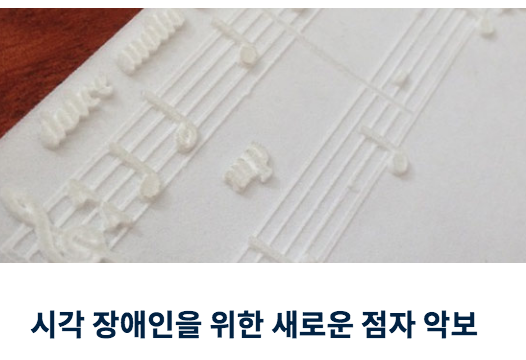
\includegraphics[width=0.7\textheight]{./image/08_05.png} \\

\includegraphics[width=0.7\textheight]{./image/08_06.png}
\end{tabular}
\end{frame}

\begin{frame}[t]{3D프린터의 미래}\footnotesize
\begin{tabular}{lcr}
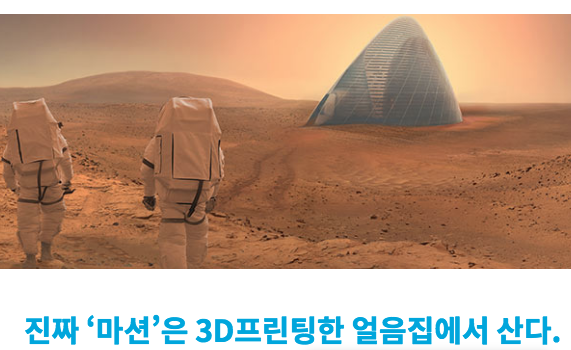
\includegraphics[width=0.7\textheight]{./image/08_07.png} \\
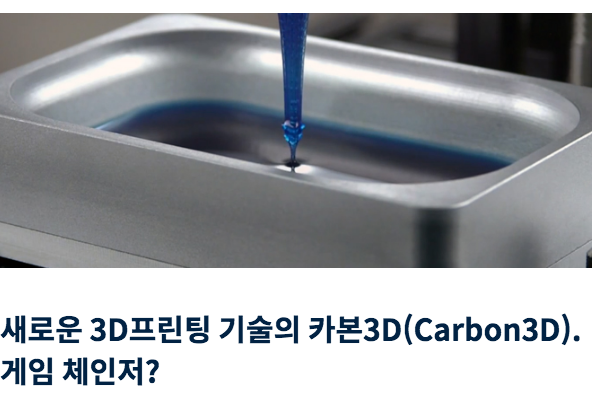
\includegraphics[width=0.7\textheight]{./image/08_08.png}
\end{tabular}
\end{frame}

\end{comment}

\section{3D Printing}

\subsection{Process}

\begin{frame}[t]{3D Printing Process}\footnotesize
\begin{tabular}{c c c}
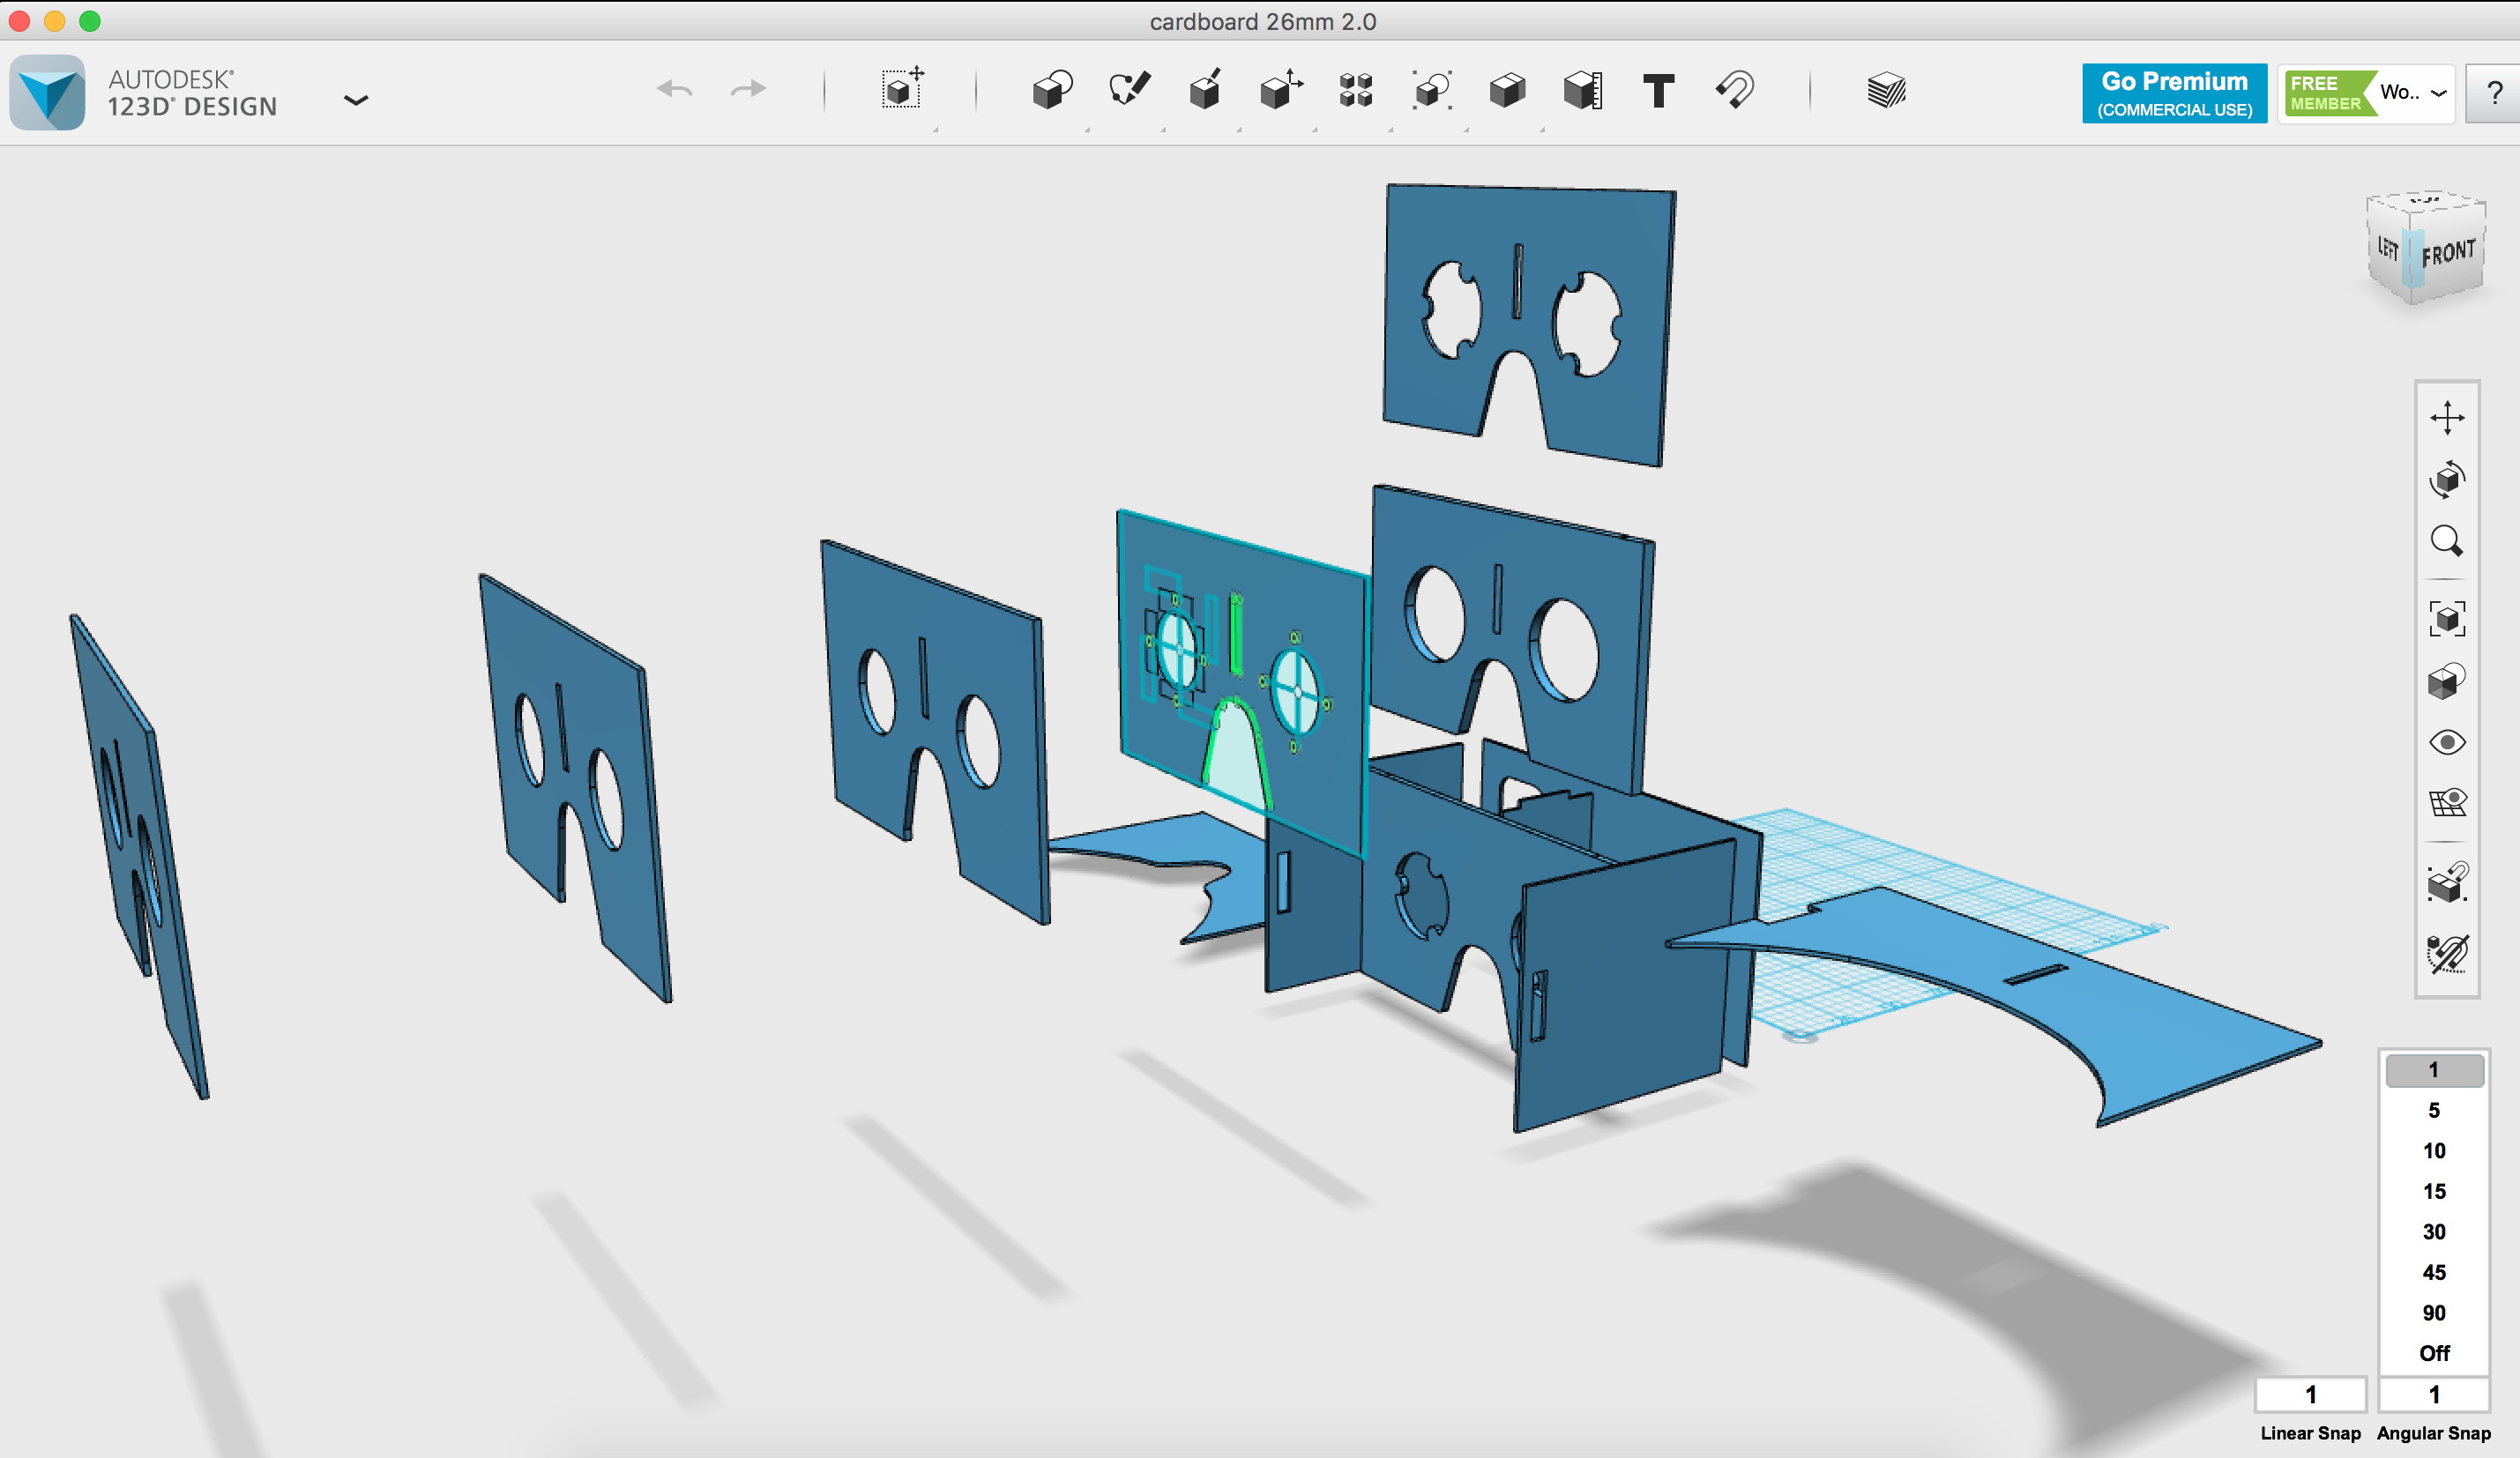
\includegraphics[width=0.4\textheight]{./image/09_01.png}&모델링(Modeling)&123d, skp 등\\ &&\\
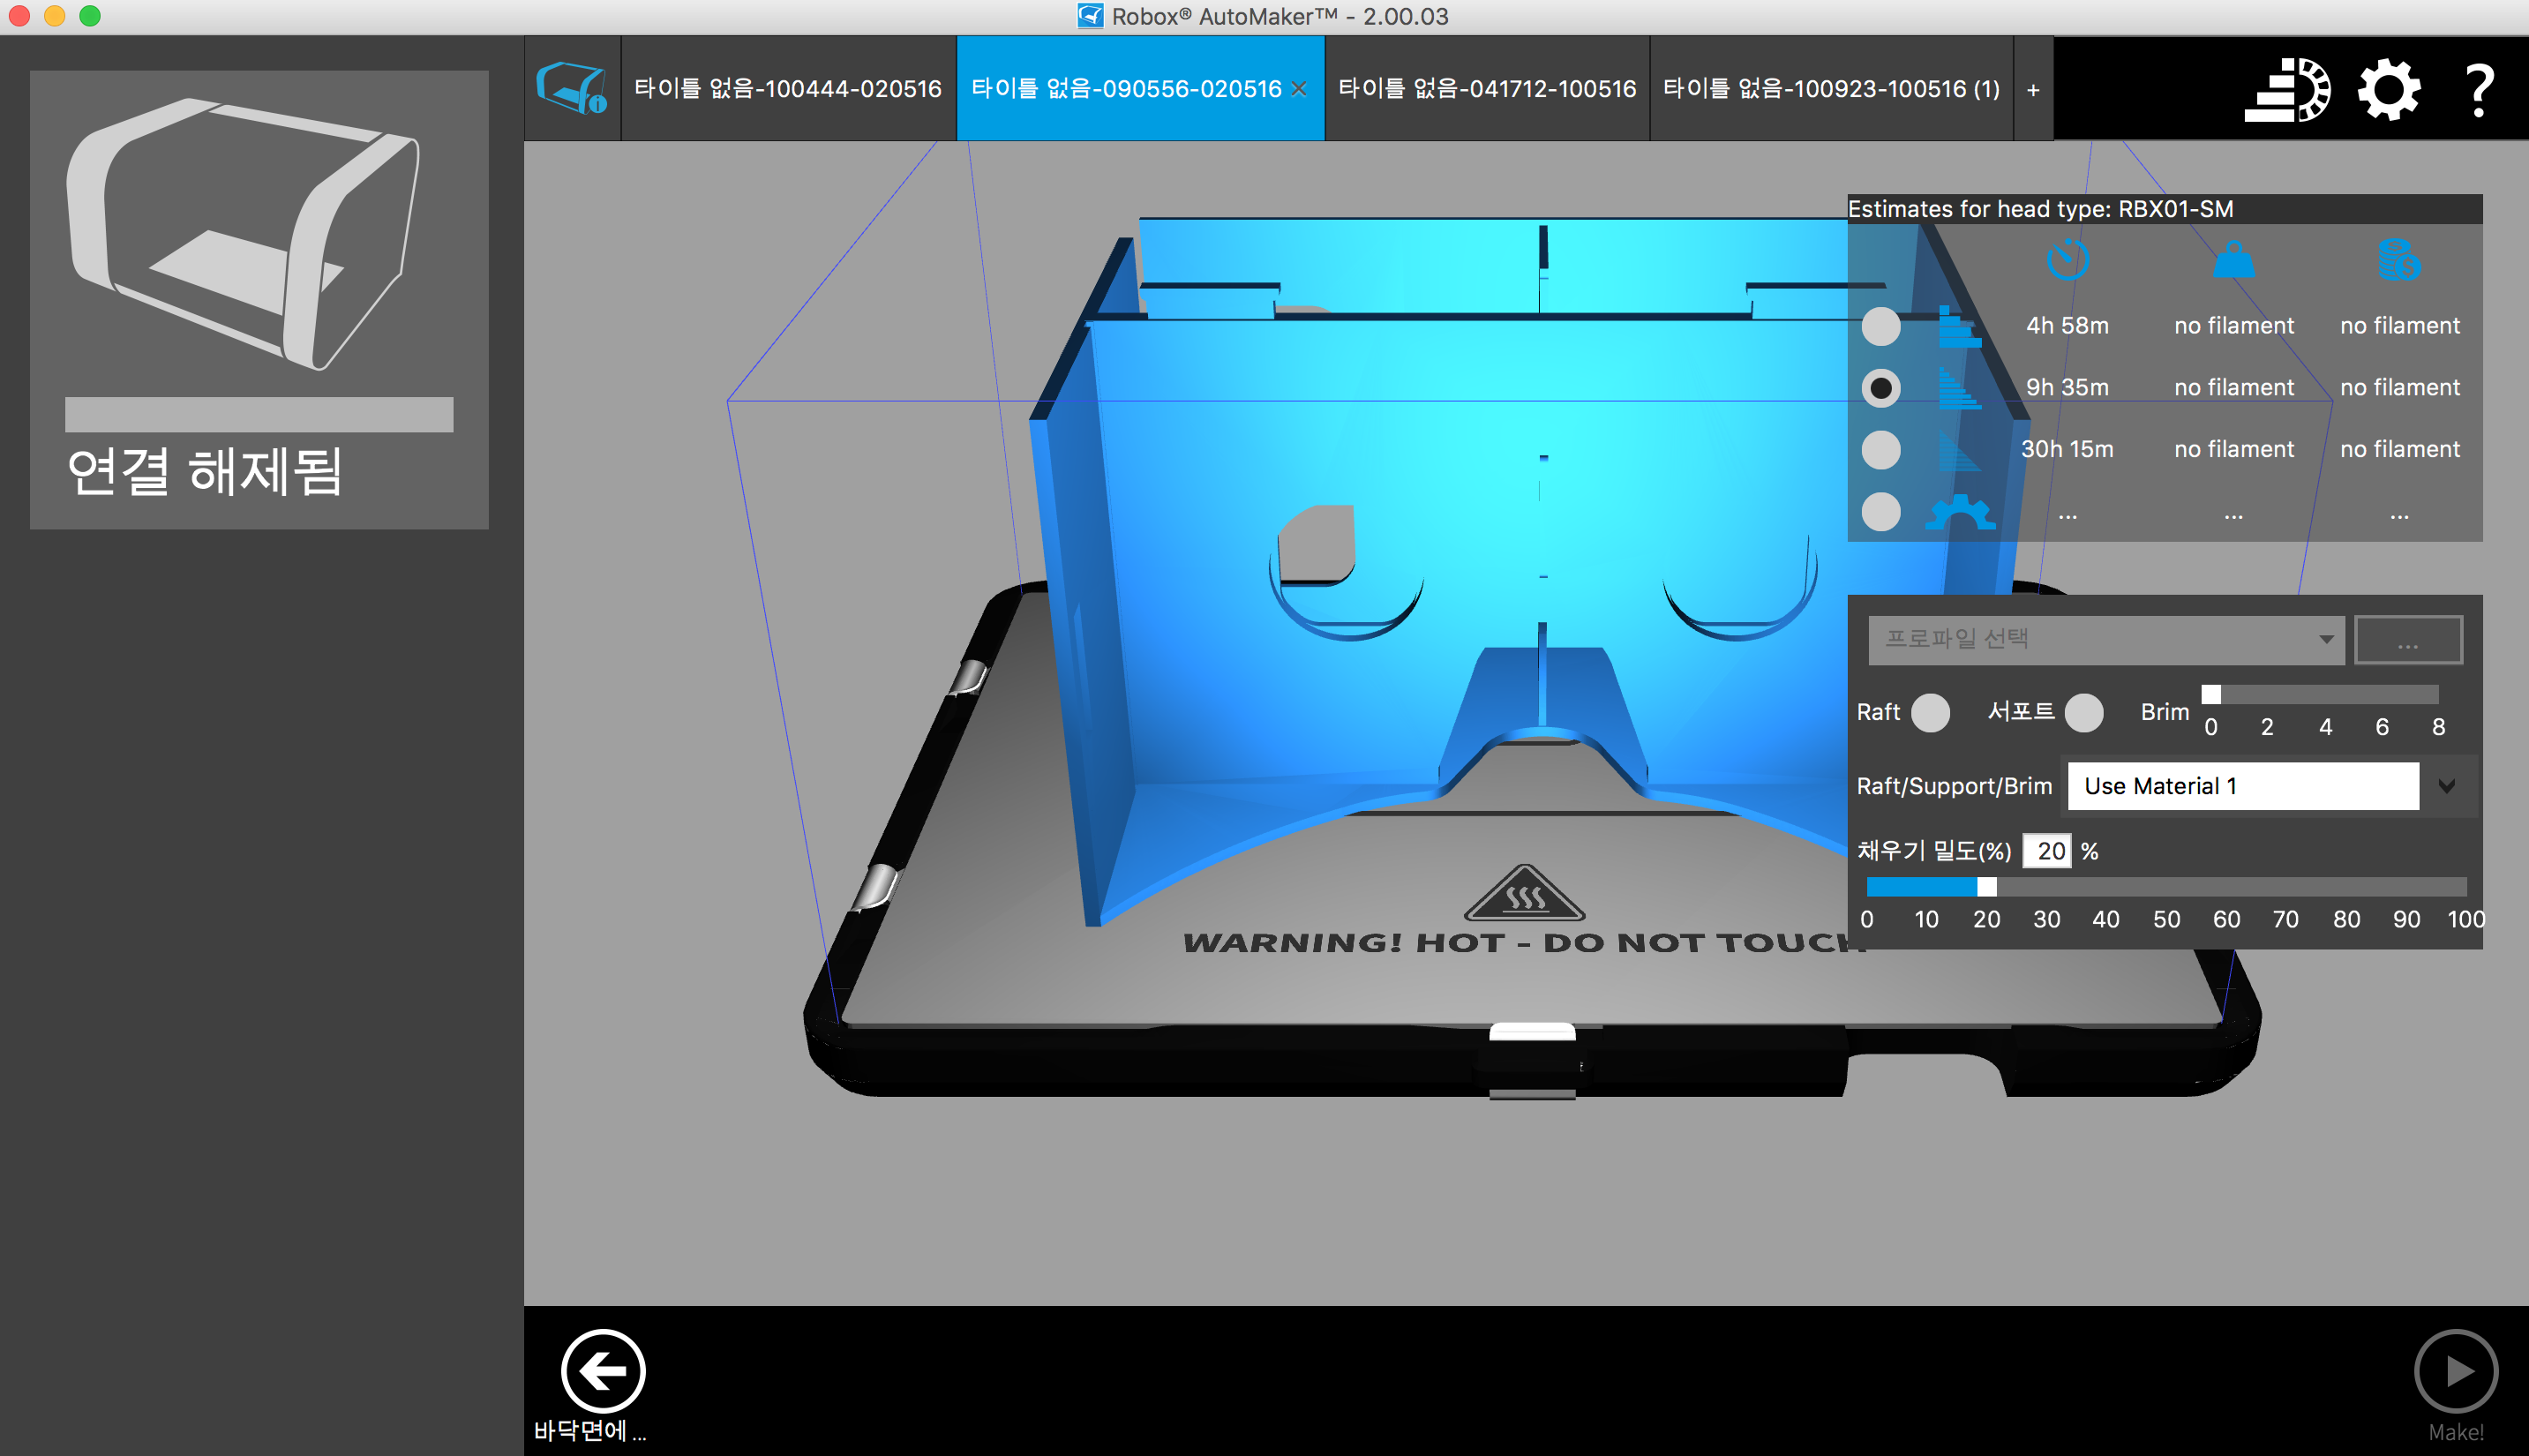
\includegraphics[width=0.4\textheight]{./image/09_02.png}&슬라이싱(Slicing)&stl, obj 등\\ &&\\
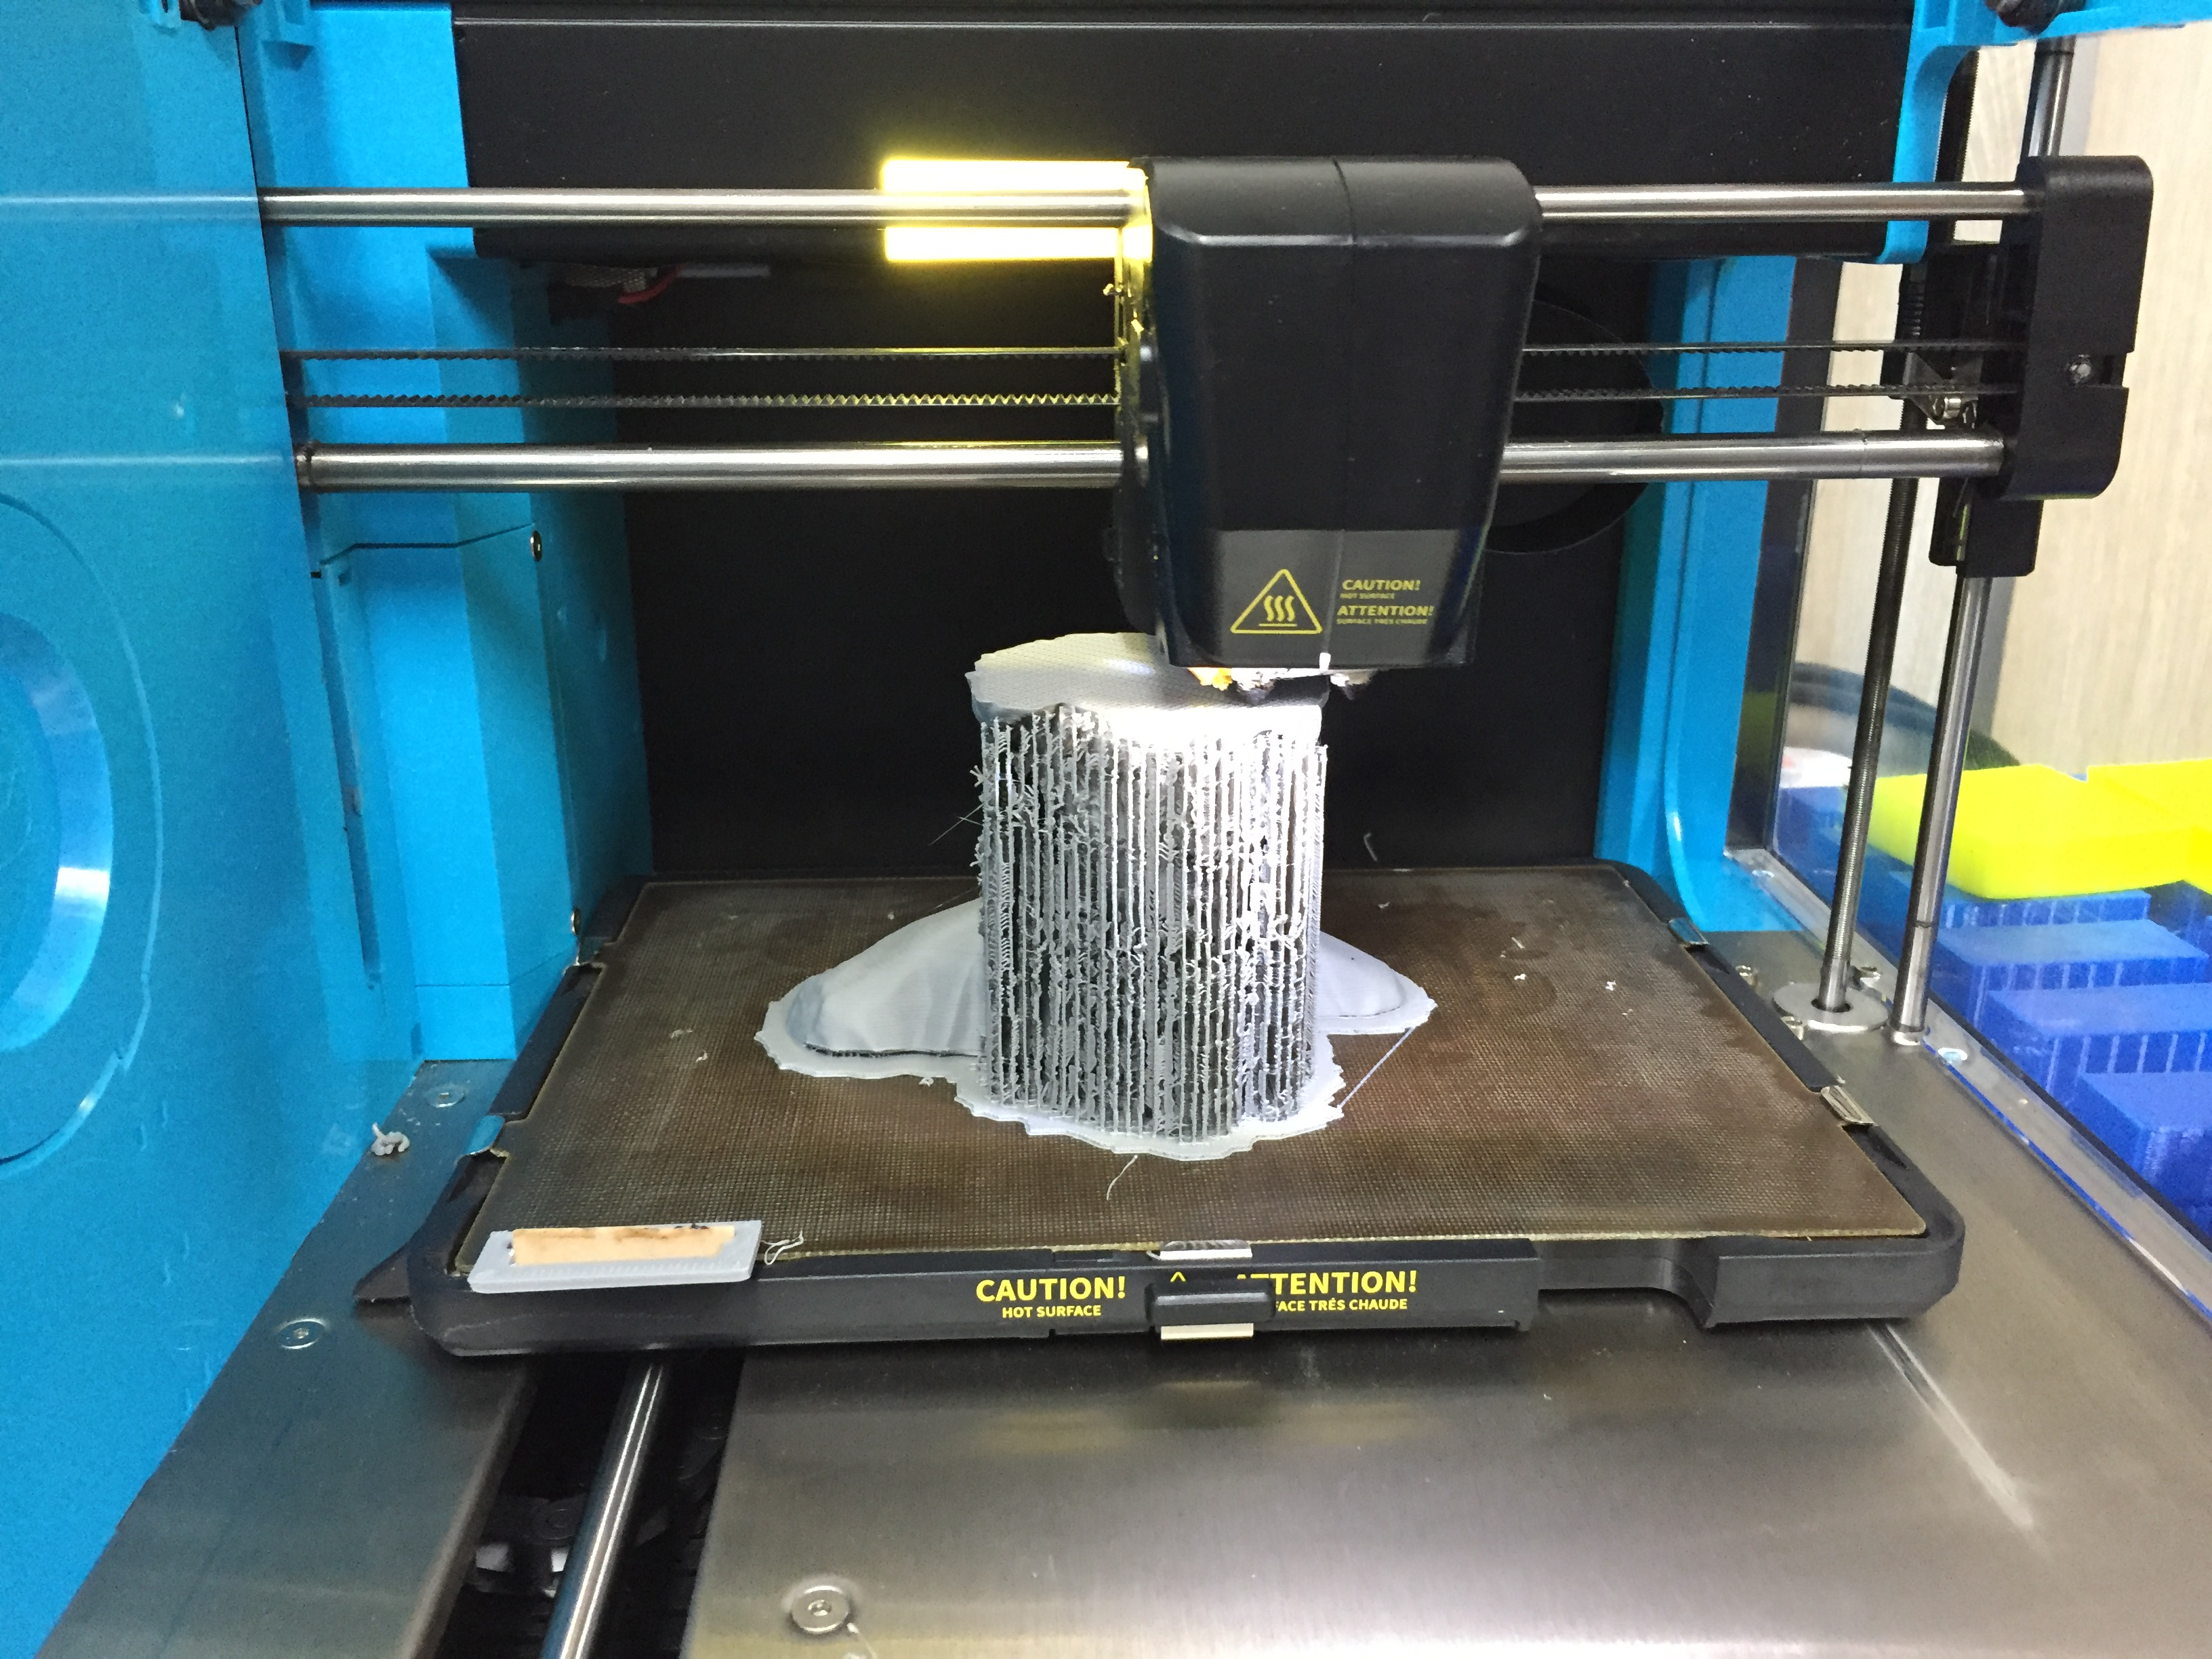
\includegraphics[width=0.4\textheight]{./image/09_03.jpg}&출력(Printing)&gcode,x3g 등
\end{tabular}
\end{frame}

\subsection{Prepare}

\begin{frame}[t]{Filament}\footnotesize
\begin{itemize}
\item ABS : 일반적인 플라스틱
\item PLA : 녹색 옥수수 가루로 만든 이쑤시게
\item HIPS, PVA : Support 재료로 많이 쓰임. 액체에 녹음
\item TPU, Flexible : 탄성이 있고 말랑말랑한 소재
\item Nylon
\item Conductive PLA : 전도성 필라멘트
\item ThermoChrome PLA
\end{itemize}
\raggedleft
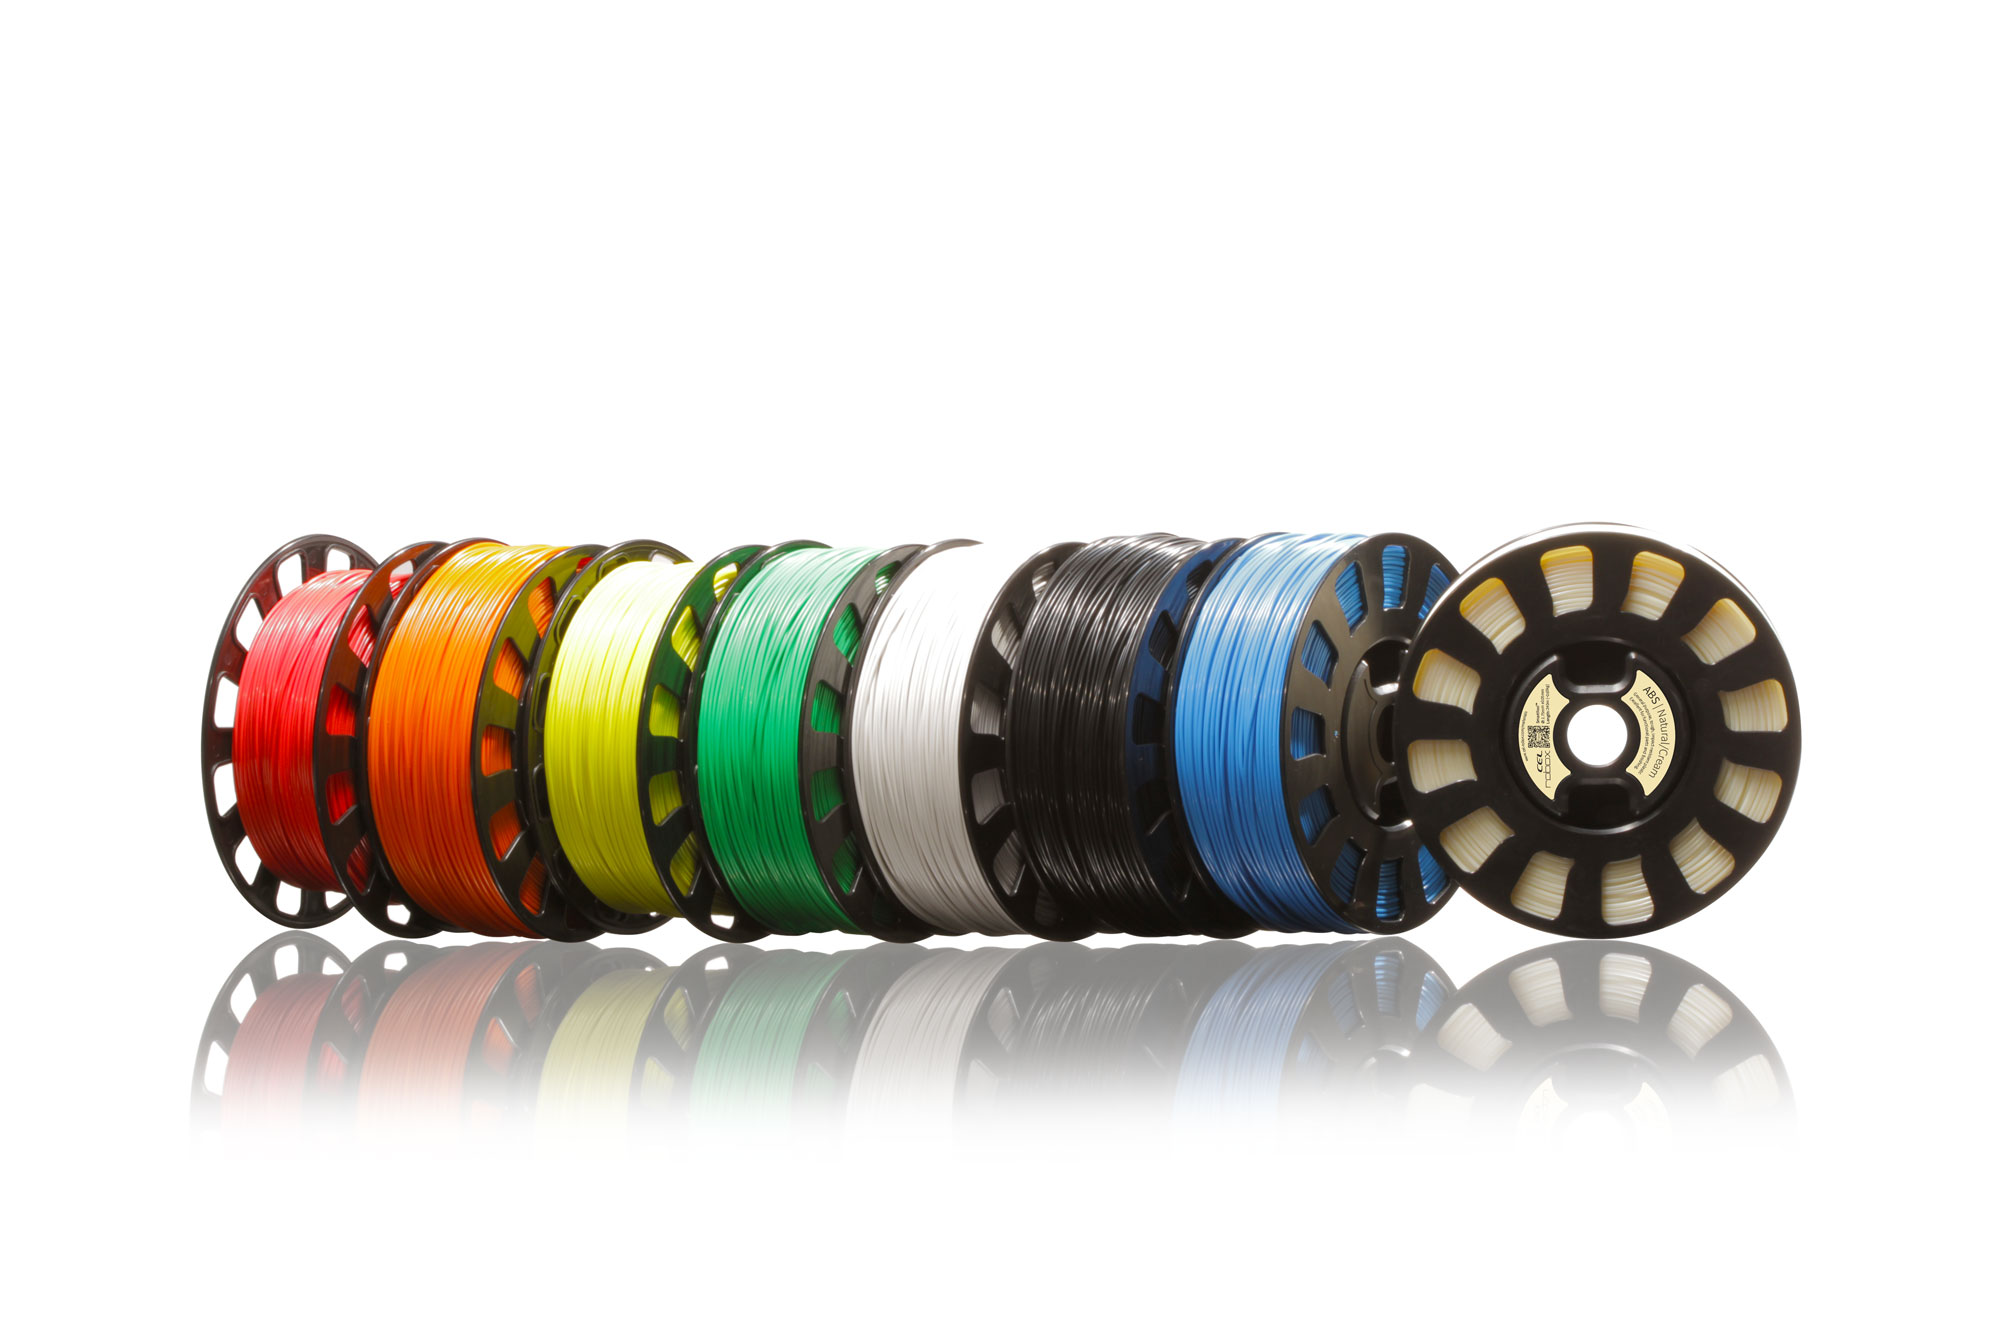
\includegraphics[width=0.7\textheight]{./image/10_01.jpg}
\end{frame}



\begin{frame}[t]{열수축(shrinkage)}\footnotesize
\begin{itemize}
\item 플라스틱이 220 까지 가열되었다 상온에서 식으면서 열수축이 발생
\item PLA보다는 ABS가 열수축이  더 많이 일어남
\item 열수축을 줄이기 위해 히팅베드(Heating Bed)와 챔버(Chamber)를 사용
\end{itemize}
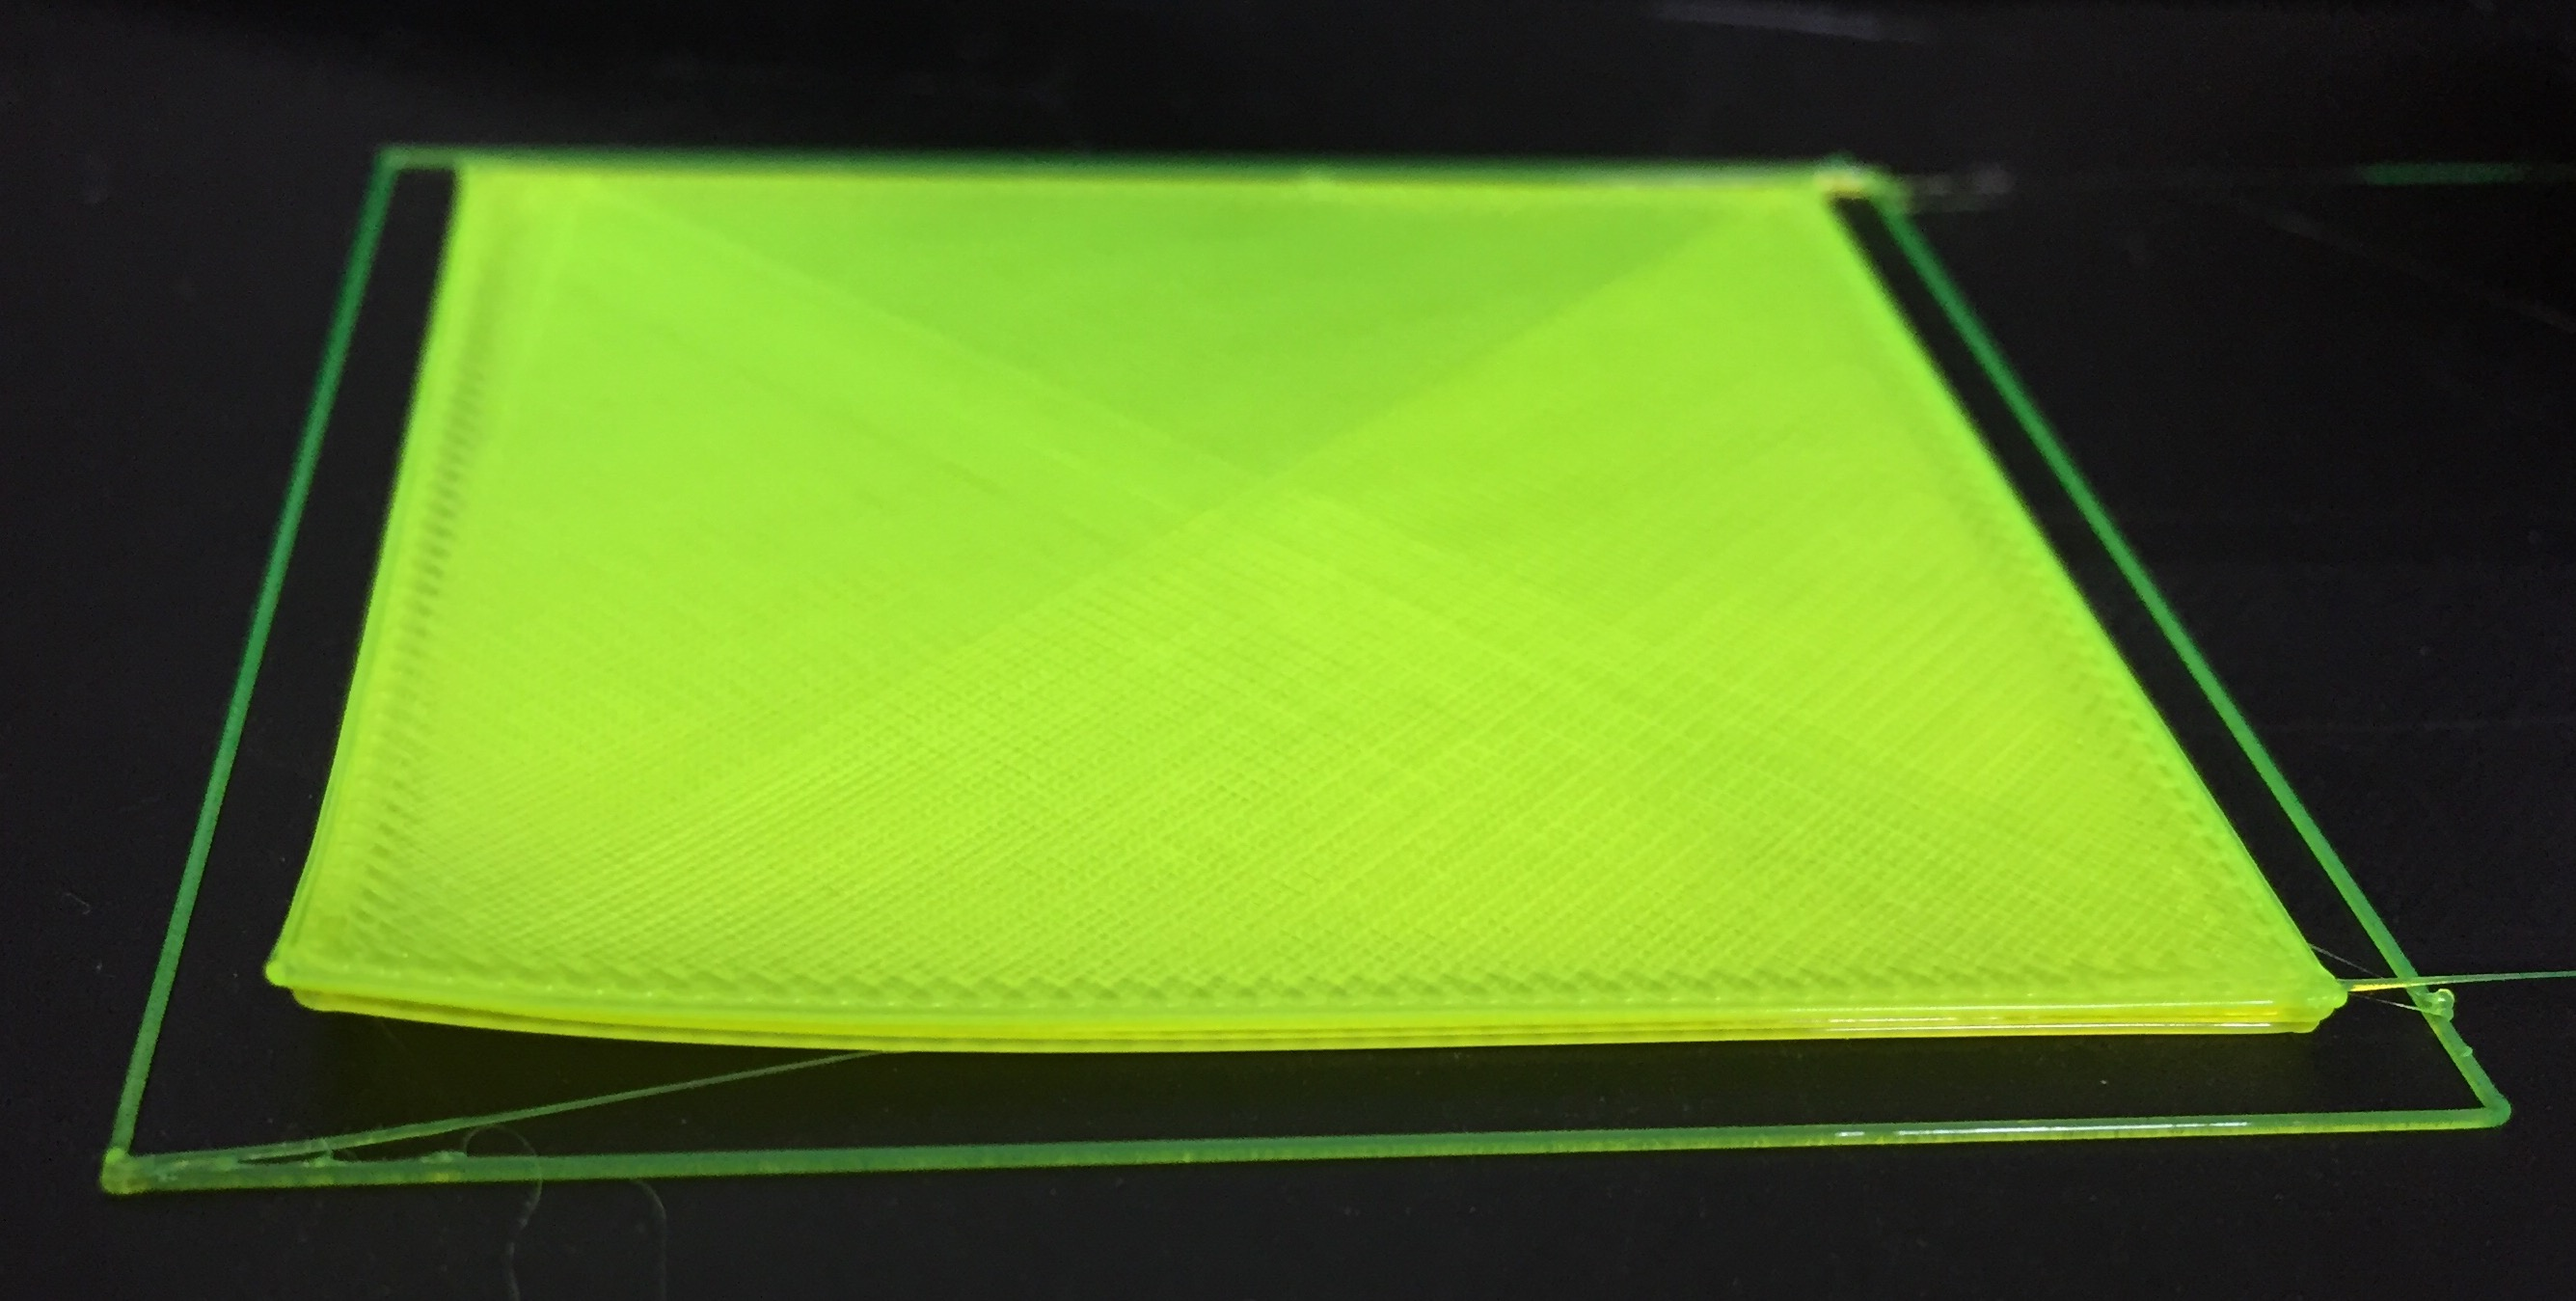
\includegraphics[width=5cm, height=2cm]{./image/11_1.JPG} \@ 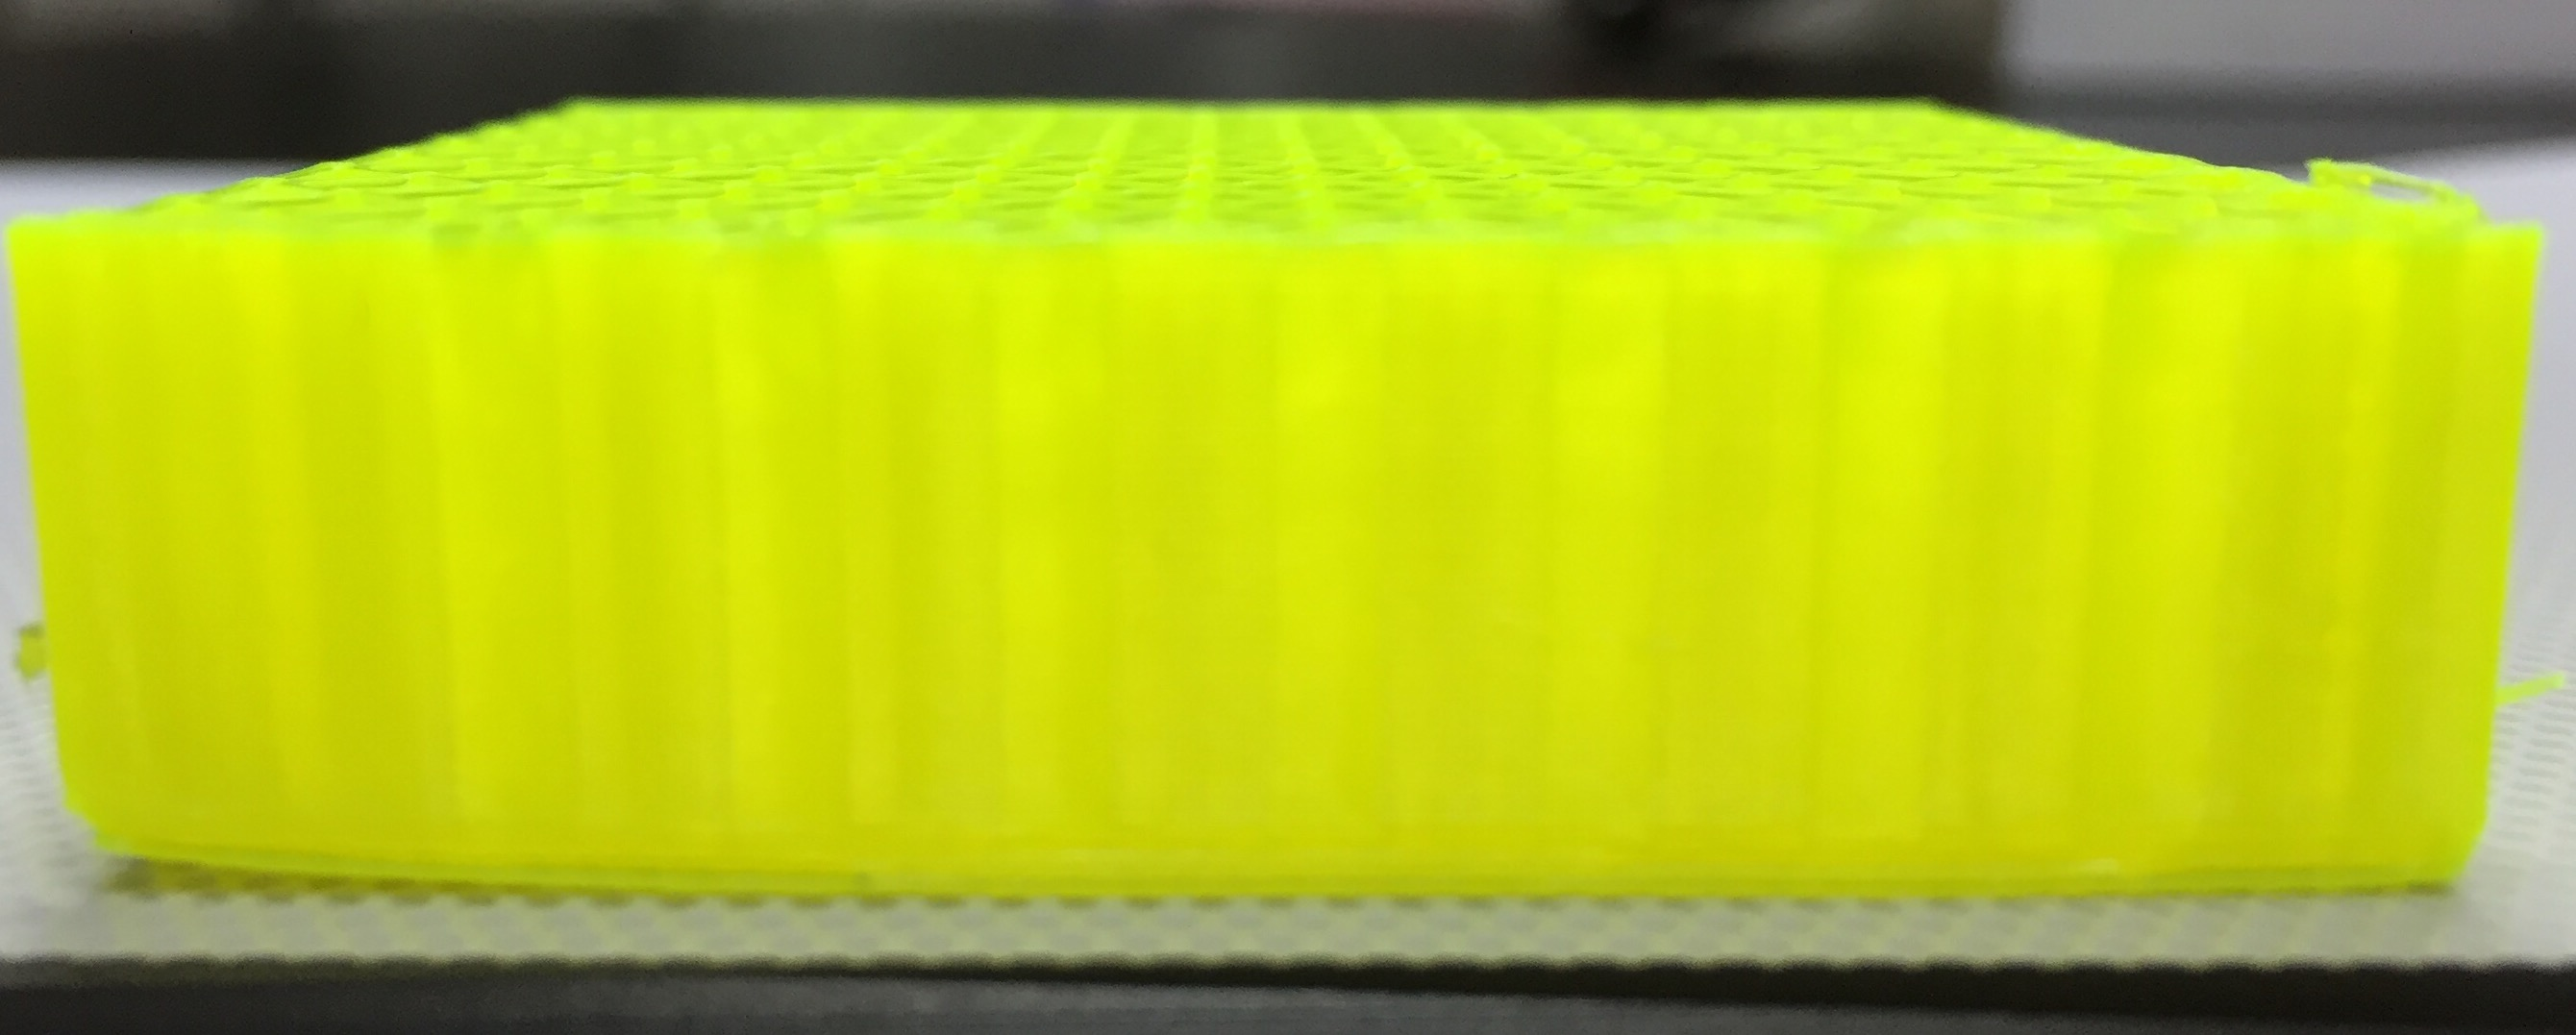
\includegraphics[width=5cm, height=2cm]{./image/11_2.JPG}
\end{frame}

\begin{frame}[t]{Support}\footnotesize
\begin{itemize}
\item 바닥부터 쌓아올라가는 방식이므로 허공에서 출력을 시작할 수 없음
\item 모델링을 할 때부터 출력을 고려해야 함
\item 슬라이싱 프로그램에서 서포트(Support)를 자동으로 생성할 수 있음
%\item 가급적 사용하지 않는 것이 좋음
\item 듀얼 익스트루더를 사용하면 서포트 재료로 HIPS나 PVA 사용
\end{itemize}
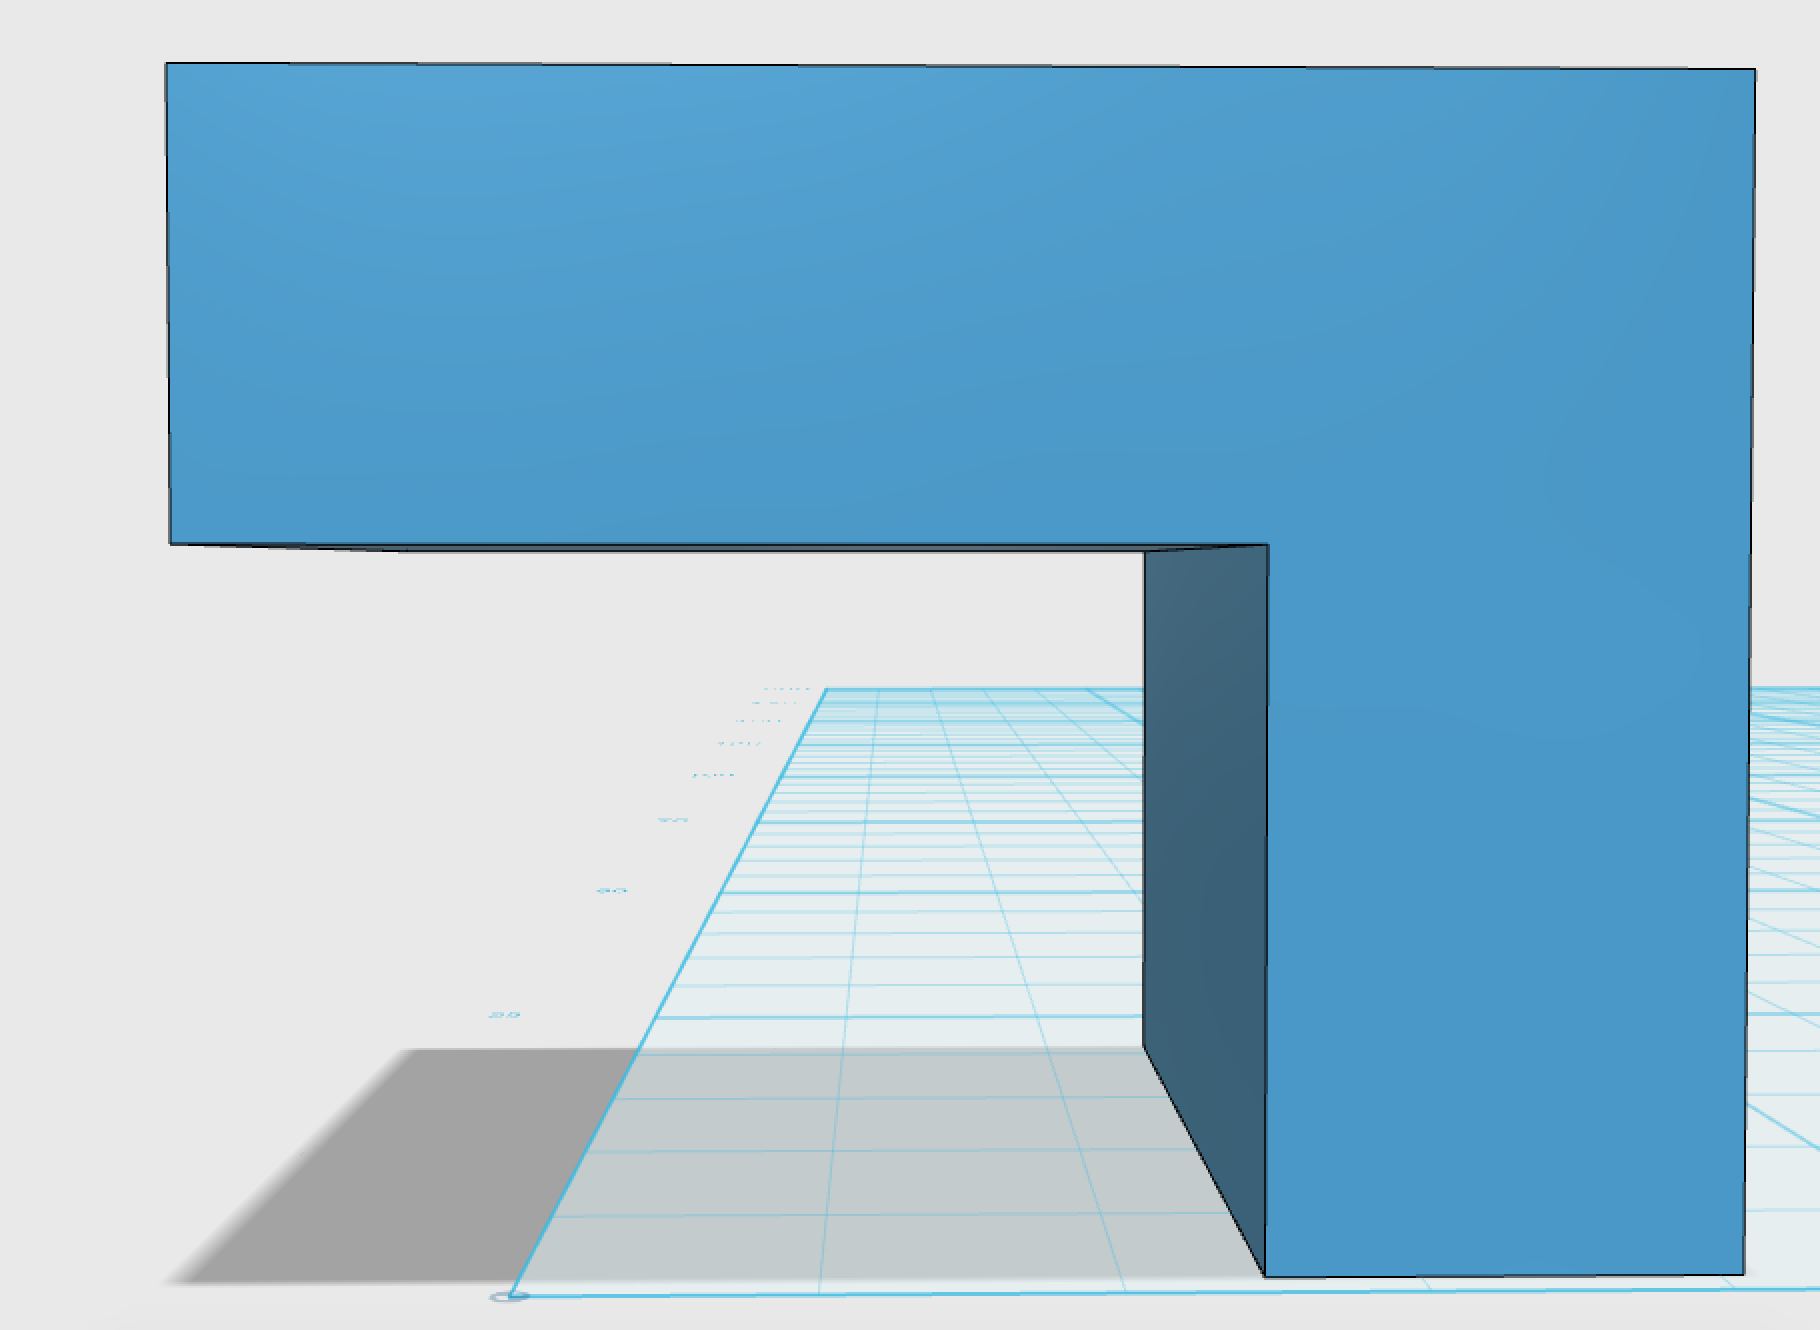
\includegraphics[width=5cm, height=3.5cm]{./image/12_01.png} \@ 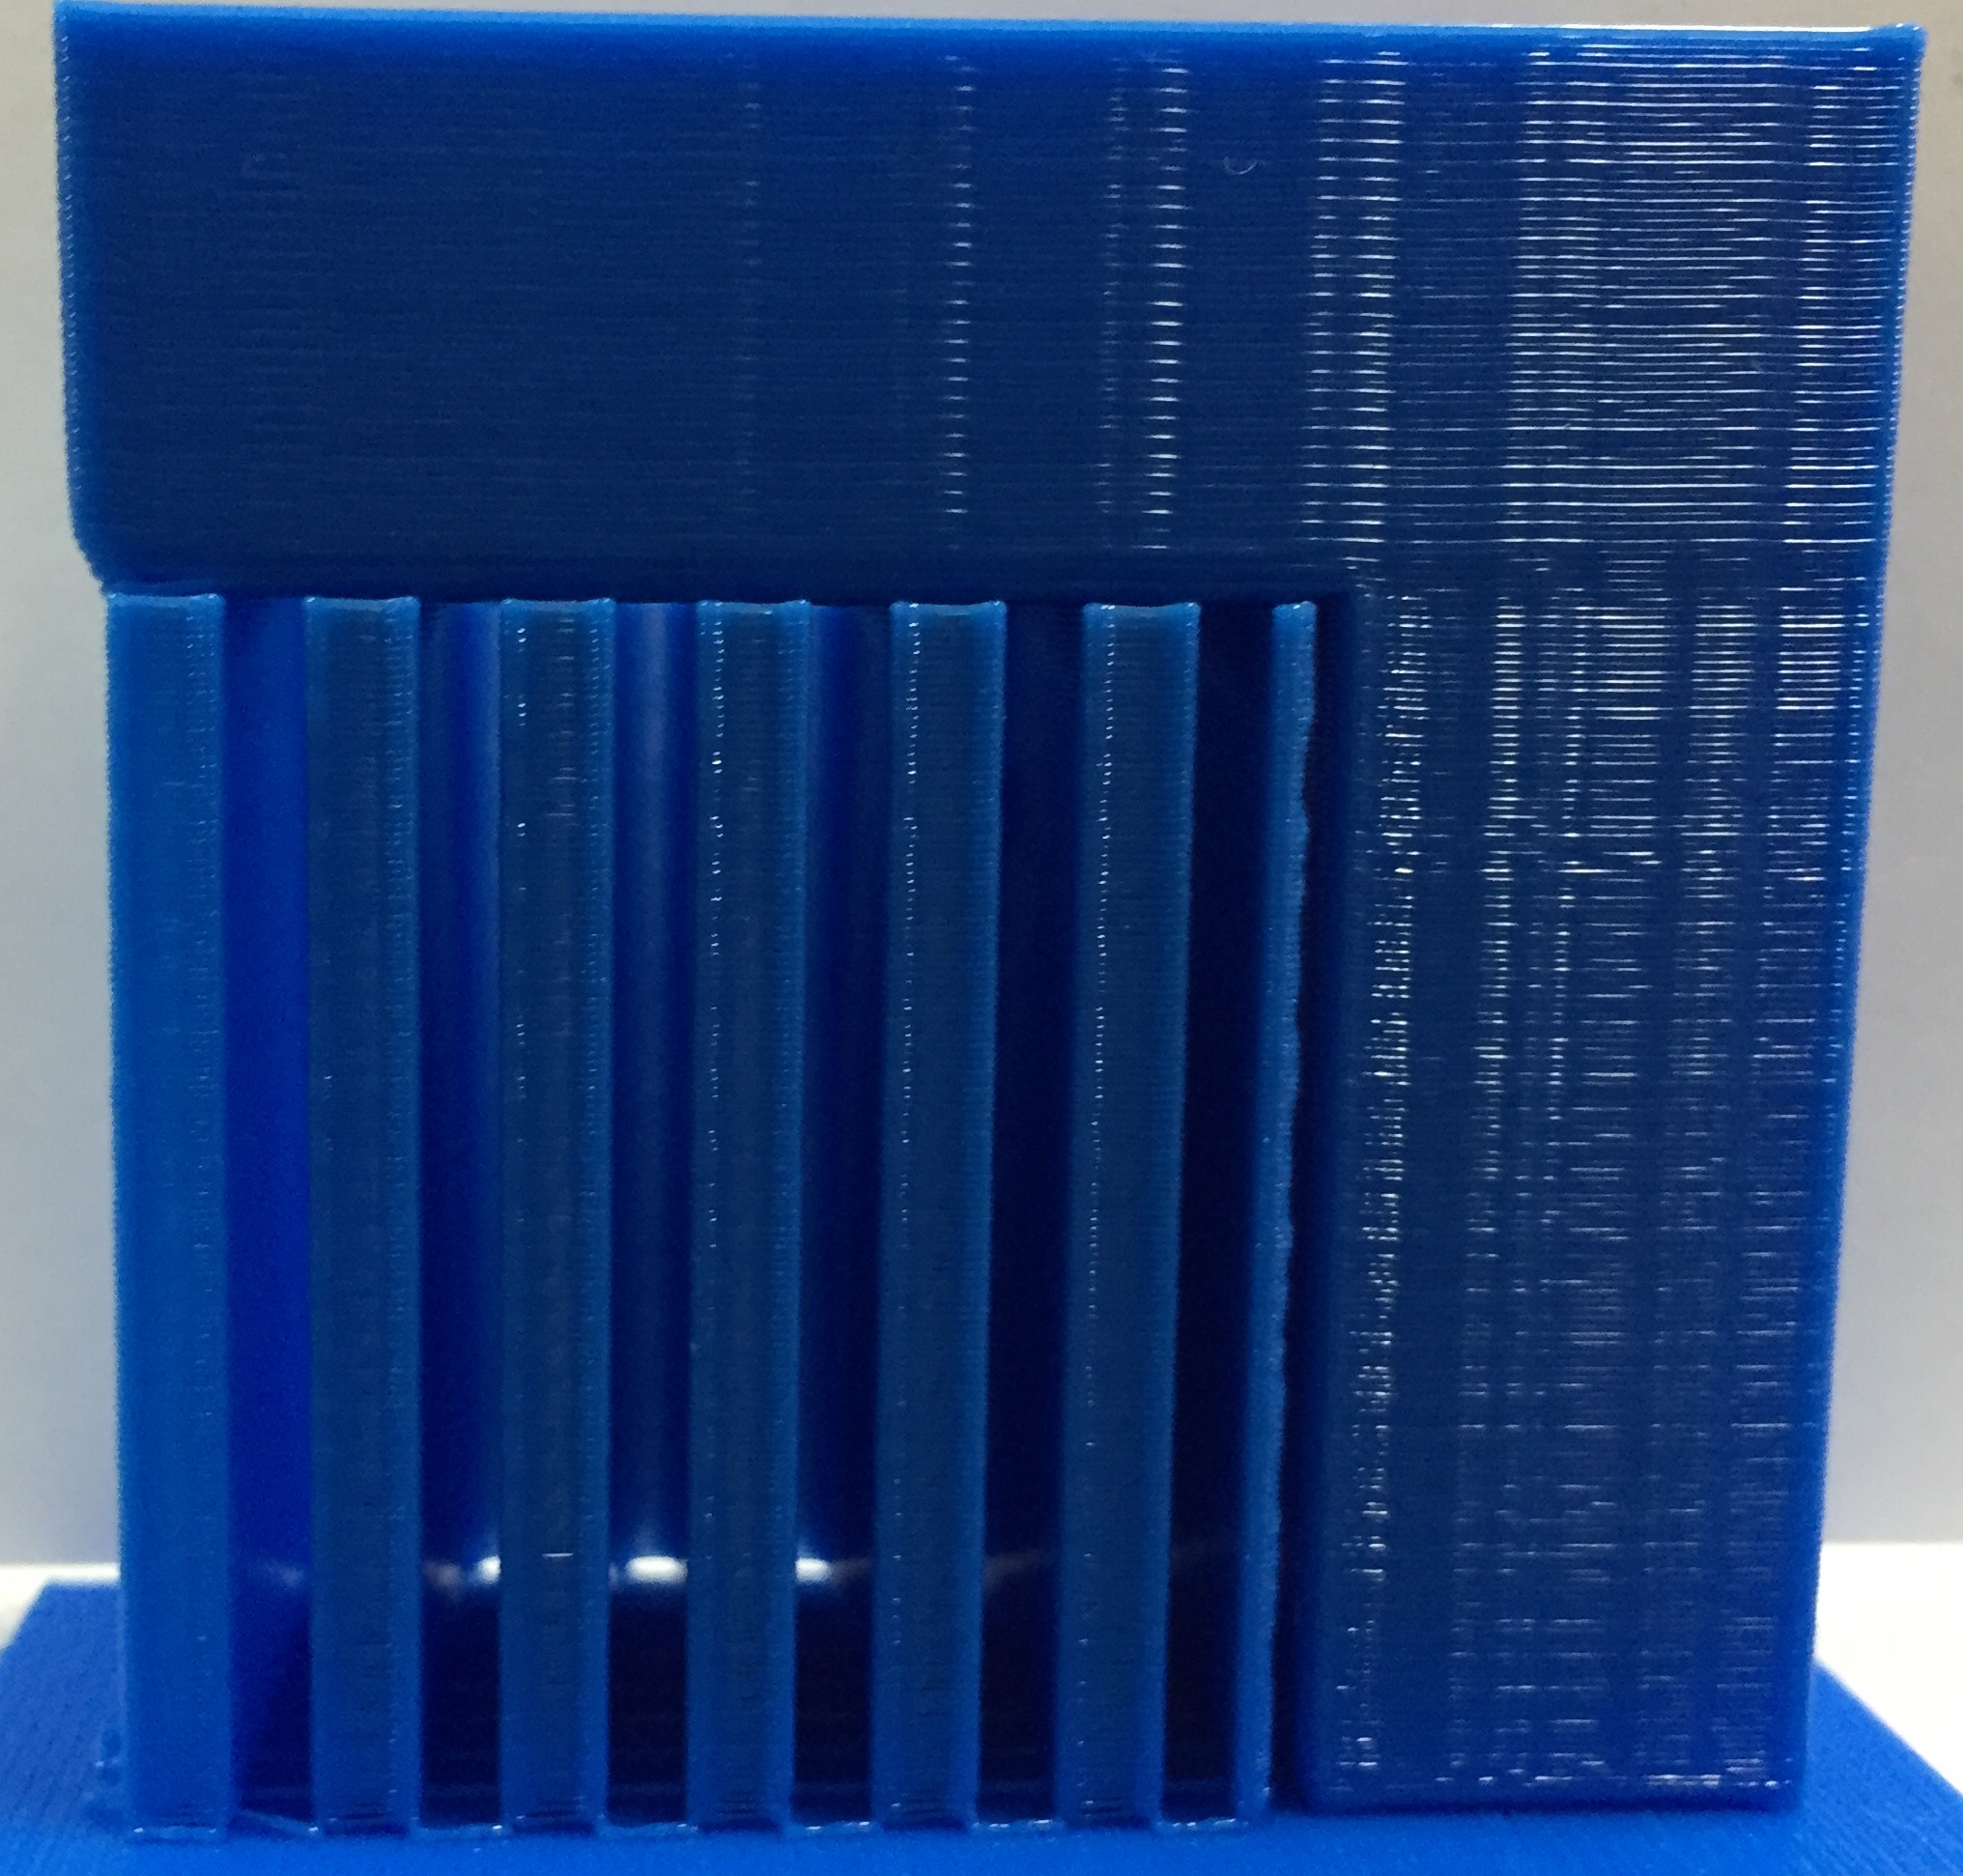
\includegraphics[width=5cm, height=3.5cm]{./image/12_02.jpg}
\end{frame}

\begin{frame}[t]{Support}\footnotesize
\begin{itemize}
\item 60도 정도는 안정되게 출력 가능
\item 최대 45도 정도까지 출력 가능
%\item 가급적 사용하지 않는 것이 좋음
\end{itemize}
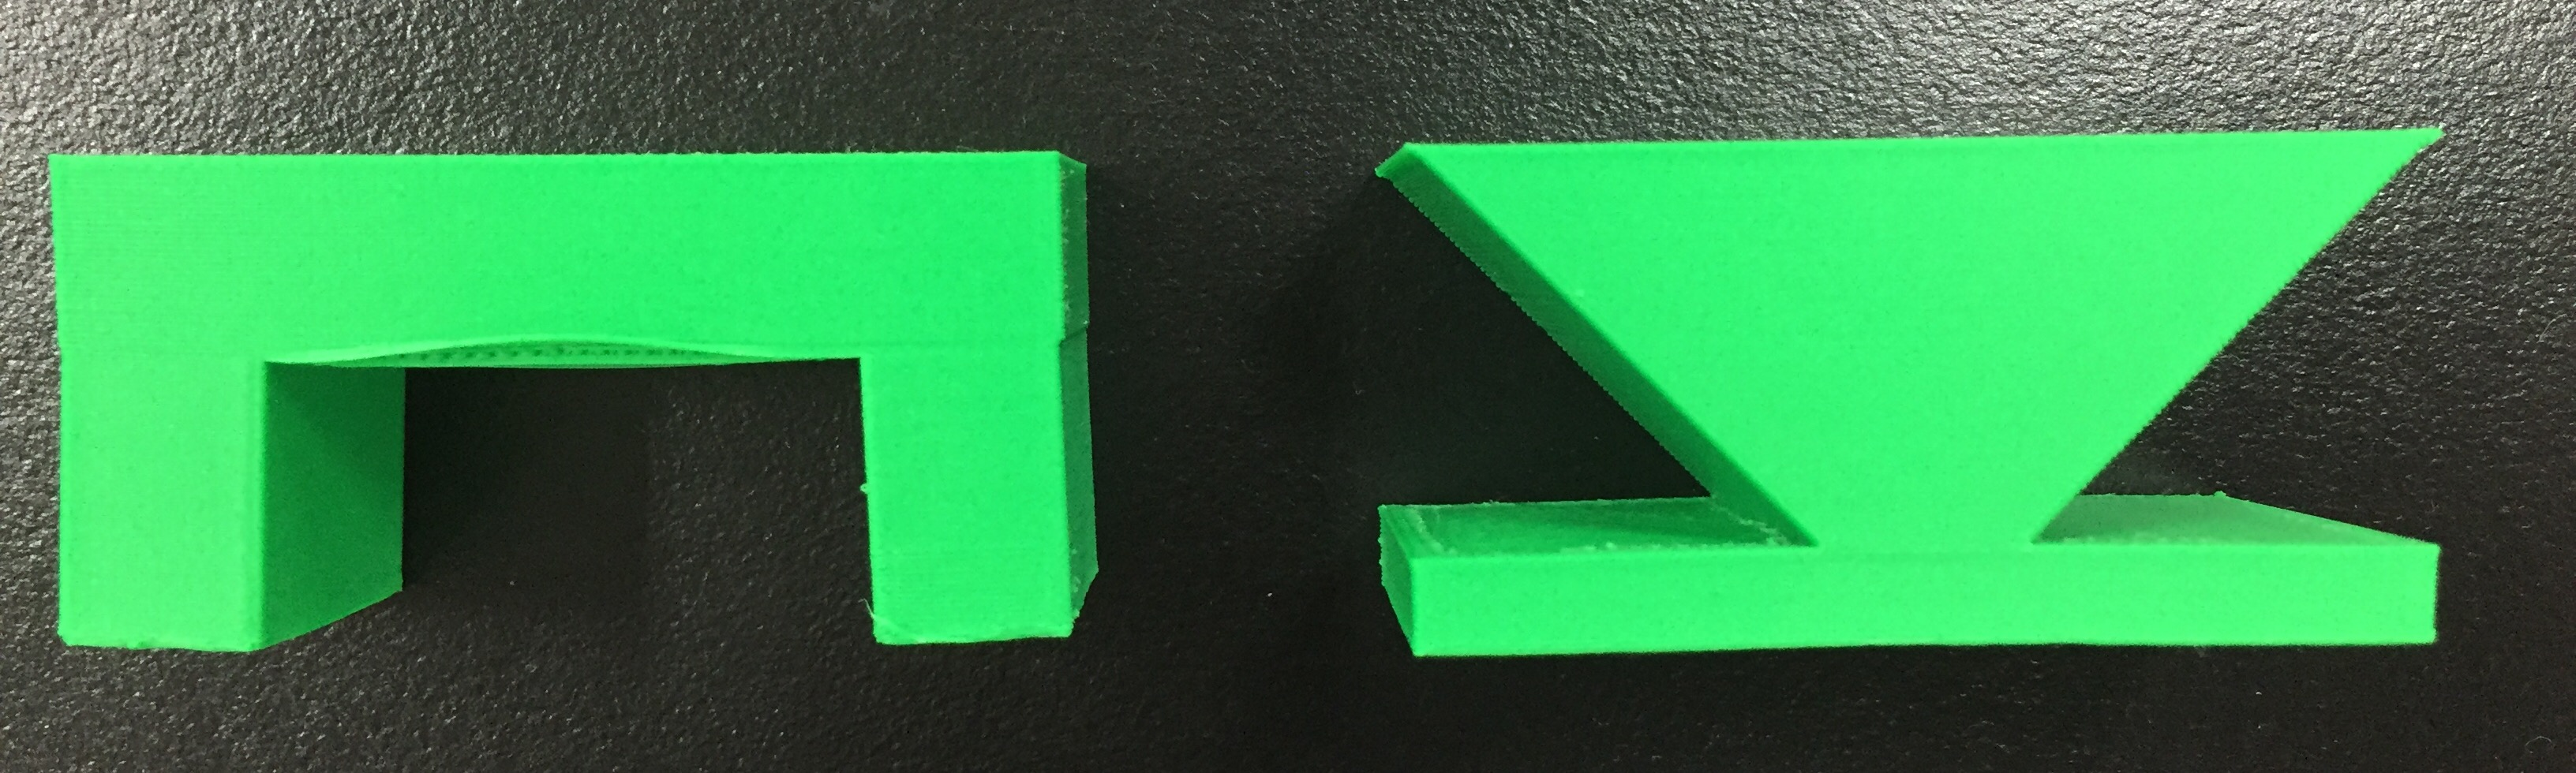
\includegraphics[width=10cm]{./image/12_03.jpg}\\
\includegraphics[width=5cm]{./image/12_04.jpg} \@ \includegraphics[width=5cm]{./image/12_05.jpg}
\end{frame}

\begin{frame}[t]{Brim and Raft}\footnotesize
\begin{itemize}
\item 출력물 바닥 면적이 작거나 Bed에 잘 붙지 않는 경우 사용
\item Brim은 한 층
\item Raft는 여러 층으로 Support를 사용할 때 함께 사용하면 좋음
\end{itemize}
\begin{tabular}{cc}
\includegraphics[width=4.5cm, height=3cm]{./image/13_01.jpg}& \includegraphics[width=4.5cm, height=3cm]{./image/13_02.jpg}\\
Brim&Raft
\end{tabular}
\end{frame}

\begin{frame}[t]{Fill}\footnotesize
\begin{itemize}
\item 출력물 채우기 정도
\item Fill 값이 높을수록 튼튼해지지만 무거워지고 열수축이 심해짐
\end{itemize}
\centering
\includegraphics[width=8cm, height=5cm]{./image/14_01.png}
\end{frame}

\subsection{Safety}
\begin{frame}[t]{주의사항}\footnotesize
\begin{tabular}{c l}
\includegraphics[width=0.4\textheight]{./image/15_01.png}&베드와 익스트루더 고온 조심\\ &\\
\includegraphics[width=0.4\textheight]{./image/15_02.png}&챔버 안 손 조심
\end{tabular}
\end{frame}


%%%%%%% 큐비콘 주의사항

\begin{frame}[t]{주의사항}\footnotesize
	\includegraphics[width=10cm]{./image/18_02.png}
\end{frame}

\begin{frame}[t]{주의사항}\footnotesize
	\includegraphics[width=10cm]{./image/18_03.png}
\end{frame}

\begin{frame}[t]{주의사항}\footnotesize
	\includegraphics[width=10cm]{./image/18_04.png}
\end{frame}


%%%%%%%%%%%%%%%%%%%%%%%
\begin{comment}

\subsection{Edison}

\begin{frame}[t]{Edison Pro}\footnotesize
\centering
\includegraphics[width=7cm]{./image/16_00.png}
\end{frame}

\begin{frame}[t]{Spec}\footnotesize
\centering
\includegraphics[width=10cm]{./image/16_04.png}
\end{frame}



\begin{frame}[t]{필라멘트 빼기}\footnotesize
\centering
\includegraphics[width=10cm]{./image/16_01.png}
\end{frame}

\begin{frame}[t]{필라멘트 넣기}\footnotesize
\centering
\includegraphics[width=10cm]{./image/16_02.png}
\end{frame}

\begin{frame}[t]{수평맞추기}\footnotesize
\centering
\includegraphics[width=10cm]{./image/16_05.png}
\end{frame}

\begin{frame}[t]{출력시작하기(듀얼노즐)}\footnotesize
\centering
\includegraphics[width=10cm]{./image/16_06.png}
\end{frame}

\begin{frame}[t]{출력시작하기(유니버설익스트루더)}\footnotesize
\centering
\includegraphics[width=10cm]{./image/16_07.png}
\end{frame}



\begin{frame}[t]{출력시작하기(싱글노즐)}\footnotesize
\centering
\includegraphics[width=10cm]{./image/16_03.png}
\end{frame}



%%%%%%%%%%%%%%%%%%%%%

\begin{frame}[t]{MakerBot}\footnotesize
\begin{itemize}
\item google에서 makerbot로 검색해 사이트에 접속
\item 자신의 운영체제에 맞는 버전을 다운로드 후 설치
\end{itemize}
\includegraphics[width=5cm, height=4cm]{./image/16_08.png} \@ \includegraphics[width=5cm, height=4cm]{./image/16_10.png}
\end{frame}

\begin{frame}[t]{MakerBot}\footnotesize
\begin{itemize}
\item makerbot desktop 실행
\item Devices  Select Type of Device → Replicator(Single)
\end{itemize}
\includegraphics[width=5cm, height=4cm]{./image/16_11.png} \@ \includegraphics[width=5cm, height=4cm]{./image/16_12.png}
\end{frame}


\begin{frame}[t]{MakerBot}\footnotesize
\begin{itemize}
\item ADD FILE
\item STL 파일 추가
\end{itemize}
\includegraphics[width=5cm, height=4cm]{./image/16_27.png} \@ \includegraphics[width=5cm, height=4cm]{./image/16_28.png}
\end{frame}

\begin{frame}[t]{MakerBot}\footnotesize
\begin{itemize}
\item Chage Position
\item On Platform, Center
\end{itemize}
\includegraphics[width=5cm, height=4cm]{./image/16_17.png} \@ \includegraphics[width=5cm, height=4cm]{./image/16_18.png}
\end{frame}

\begin{frame}[t]{MakerBot}\footnotesize
\begin{itemize}
\item Change Rotation
\item Support를 사용하지 않을 수 있도록 각도 조정
\end{itemize}
\includegraphics[width=5cm, height=4cm]{./image/16_19.png} \@ \includegraphics[width=5cm, height=4cm]{./image/16_20.png}
\end{frame}

\begin{frame}[t]{MakerBot}\footnotesize
\begin{itemize}
\item Change Dimensions
\item Uniform scaling
\end{itemize}
\includegraphics[width=10cm, height=5cm]{./image/16_22.png}
\end{frame}

\begin{frame}[t]{MakerBot}\footnotesize
\begin{itemize}
\item SETTINGS
\item Quality : Low, Material : PLA
\end{itemize}
\includegraphics[width=10cm, height=5cm]{./image/16_23.png}
\end{frame}

\begin{frame}[t]{MakerBot}\footnotesize
\begin{itemize}
\item PREVIEW
\item 출력시간과 재료소모량 확인
\item 출력 시간이 10분 안쪽이 되도록 크기 재 조정
\end{itemize}
\includegraphics[width=10cm, height=5cm]{./image/16_25.png}
\end{frame}

\begin{frame}[t]{MakerBot}\footnotesize
\begin{itemize}
\item Export
\item X3G로 저장 후 SD카드에 복사  → 3D프린터에서 출력
\end{itemize}
\includegraphics[width=10cm, height=5cm]{./image/16_26.png}
\end{frame}


\begin{frame}[t]{CreatorK}\footnotesize
\begin{itemize}
\item http://www.3disonprinter.com/ → Support → Download 에서 CreatorK를 다운받아 설치 
\item CreatorK를 실행
\item 장비설정 : 프린터 → 프린터타입 → The 3DISON PRO 
\end{itemize}
\includegraphics[width=10cm, height=4.5cm]{./image/16_29.png}
\end{frame}

\begin{frame}[t]{CreatorK}\footnotesize
\begin{itemize}
\item STL파일 불러오기
\item 파일 → 열기 → STL 파일 찾아 불러오기
\end{itemize}
\includegraphics[width=5cm]{./image/16_30.png} \@ \includegraphics[width=5cm]{./image/16_31.png}
\end{frame}

\begin{frame}[t]{CreatorK}\footnotesize
\begin{itemize}
\item 모델 회전하기
\item 출력하기 좋은 방향으로 회전
\end{itemize}
\includegraphics[width=5cm]{./image/16_34.png} \@ \includegraphics[width=5cm]{./image/16_35.png}
\end{frame}

\begin{frame}[t]{CreatorK}\footnotesize
\begin{itemize}
\item 플랫폼 가운데 놓기
\end{itemize}
\includegraphics[width=5cm]{./image/16_32.png} \@ \includegraphics[width=5cm]{./image/16_33.png}
\end{frame}

\begin{frame}[t]{CreatorK}\footnotesize
\begin{itemize}
\item G-Code 생성
\item 베이스/서포터사용 안함, 채우기 10
\end{itemize}
\includegraphics[width=5cm]{./image/16_36.png} \@ \includegraphics[width=5cm]{./image/16_37.png}
\end{frame}

\begin{frame}[t]{CreatorK}\footnotesize
\begin{itemize}
\item X3G 생성
\end{itemize}
\includegraphics[width=5cm]{./image/16_38.png} \@ \includegraphics[width=5cm]{./image/16_39.png}
\end{frame}



\end{comment}
%%%%%%%%%%%%%%%%%%%%%%%%%%%
%\begin{comment}
\subsection{Robox}

\begin{frame}[t]{Robox}\footnotesize
\centering
\includegraphics[width=8cm]{./image/17_00.jpg}
\end{frame}

\begin{frame}[t]{Spec}\footnotesize
\includegraphics[width=8cm]{./image/17_01.png}\\
\raggedleft
\includegraphics[width=4cm]{./image/17_08.png}
\end{frame}

\begin{frame}[t]{Overview}\footnotesize
\centering
\includegraphics[width=5cm, height=3.5cm]{./image/17_02.png}
\includegraphics[width=5cm, height=3.5cm]{./image/17_03.png}
\end{frame}

\begin{frame}[t]{Software Install}\footnotesize
\begin{itemize}
\item Robox, http://www.cel-robox.com/ 에서 OS에 맞는 소프트웨어 다운로드 및 설치
\end{itemize}
\centering
\includegraphics[width=8cm]{./image/17_14.png}
\end{frame}

\begin{frame}[t]{Loading Filament}\footnotesize
\begin{tabular}{c l}
\includegraphics[width=0.2\textheight]{./image/17_09.png}&필라멘트 끝 자르기\\ &\\
\includegraphics[width=0.35\textheight]{./image/17_10.png}&필라멘트 밀어넣기 \\ &\\
\includegraphics[width=0.35\textheight]{./image/17_11.png}&필라멘트롤 끼우기 \\ 
\end{tabular}
\end{frame}

\begin{frame}[t]{Unloading Filament}\footnotesize
\begin{tabular}{c l}
\includegraphics[width=0.5\textheight]{./image/17_26.png}&AutoMaker에서 필라멘트 제거\\ &\\
\includegraphics[width=0.5\textheight]{./image/17_13.png}&필라멘트 롤 제거 
\end{tabular}
\end{frame}

\begin{frame}[t]{AutoMaker}\footnotesize
\centering
\includegraphics[width=10cm]{./image/17_15.png}
\end{frame}

\begin{frame}[t]{AutoMaker : layout}\footnotesize
\centering
\includegraphics[width=5cm, height=3.5cm]{./image/17_20.png} \@ \includegraphics[width=5cm, height=3.5cm]{./image/17_17.png}\\
\includegraphics[width=5cm, height=3.5cm]{./image/17_18.png} \@ \includegraphics[width=5cm, height=3.5cm]{./image/17_19.png}
\end{frame}

\begin{frame}[t]{AutoMaker : Setting}\footnotesize
\centering
\includegraphics[width=10cm]{./image/17_21.png}
\end{frame}

\begin{frame}[t]{AutoMaker : Setting}\footnotesize
\centering
\includegraphics[width=10cm, height=2cm]{./image/17_07.png}\\
\includegraphics[width=10cm, height=2cm]{./image/17_06.png}\\
\includegraphics[width=10cm, height=2cm]{./image/17_05.png}
\end{frame}

\begin{frame}[t]{AutoMaker : Setting}\footnotesize
\centering
\includegraphics[width=10cm]{./image/17_23.png}
\end{frame}

\begin{frame}[t]{AutoMaker : Make}\footnotesize
\centering
\includegraphics[width=10cm]{./image/17_24.png}
\end{frame}

\begin{frame}[t]{Button}\footnotesize
\centering
\includegraphics[width=10cm]{./image/17_04.png}
\end{frame}

\begin{frame}[t]{AutoMaker : 교정 }\footnotesize
\begin{itemize}
\item 프린트의 위치를 옮기거나 AS 후, 또는 출력이 잘 되지 않을 때
\end{itemize}
\includegraphics[width=5cm, height=4cm]{./image/17_27.png} \@ \includegraphics[width=5cm, height=4cm]{./image/17_28.png}
\end{frame}

\begin{frame}[t]{AutoMaker : 교정 }\footnotesize
\begin{itemize}
\item 노즐 오프닝
\end{itemize}
\includegraphics[width=10cm, height=4cm]{./image/17_30.png}
\end{frame}

\begin{frame}[t]{AutoMaker : 교정 }\footnotesize
\begin{itemize}
\item 노즐 오프닝
\end{itemize}
\includegraphics[width=5cm, height=4cm]{./image/17_35.png} \@ \includegraphics[width=5cm, height=4cm]{./image/17_37.png}
\end{frame}

\begin{frame}[t]{AutoMaker : 교정 }\footnotesize
\begin{itemize}
\item 노즐 오프닝
\end{itemize}
\includegraphics[width=5cm, height=4cm]{./image/17_38.png} \@ \includegraphics[width=5cm, height=4cm]{./image/17_39.png}
\end{frame}

\begin{frame}[t]{AutoMaker : 교정 }\footnotesize
\begin{itemize}
\item 노즐오프닝
\end{itemize}
\includegraphics[width=5cm, height=4cm]{./image/17_40.png} \@ \includegraphics[width=5cm, height=4cm]{./image/17_41.png}
\end{frame}

\begin{frame}[t]{AutoMaker : 교정 }\footnotesize
\begin{itemize}
\item 노즐 높이
\end{itemize}
\includegraphics[width=10cm, height=4cm]{./image/17_31.png} 
\end{frame}

\begin{frame}[t]{AutoMaker : 교정 }\footnotesize
\begin{itemize}
\item 노즐 높이
\end{itemize}
\includegraphics[width=5cm, height=4cm]{./image/17_44.png} \@ \includegraphics[width=5cm, height=4cm]{./image/17_45.png}
\end{frame}

\begin{frame}[t]{AutoMaker : 교정 }\footnotesize
\begin{itemize}
\item 노즐 높이
\end{itemize}
\includegraphics[width=5cm, height=4cm]{./image/17_46.png} \@ \includegraphics[width=5cm, height=4cm]{./image/17_47.png}
\end{frame}

\begin{frame}[t]{AutoMaker : 교정 }\footnotesize
\begin{itemize}
\item 노즐 높이
\item A4 종이를 밀었을 때 밀리는 순간!
\end{itemize}
\includegraphics[width=5cm, height=4cm]{./image/17_50.png} \@ \includegraphics[width=5cm, height=4cm]{./image/17_51.png}
\end{frame}



\begin{frame}[t]{AutoMaker : 교정 }\footnotesize
\begin{itemize}
\item 노즐 배열
\end{itemize}
\includegraphics[width=10cm, height=4cm]{./image/17_32.png}
\end{frame}

\begin{frame}[t]{AutoMaker : 교정 }\footnotesize
\begin{itemize}
\item 노즐 배열
\end{itemize}
\includegraphics[width=5cm, height=4cm]{./image/17_55.png} \@ \includegraphics[width=5cm, height=4cm]{./image/17_56.png}
\end{frame}


\begin{frame}[t]{AutoMaker : 소재 퍼지 }\footnotesize
\begin{itemize}
\item 헤드에 있는 소재를 청소
\end{itemize}
\includegraphics[width=10cm, height=4cm]{./image/17_33.png}
\end{frame}



%%%%%%%%%%%%%%%%%
%%%%%큐비콘

\subsection{Cubicon}

\begin{frame}[t]{Cubicon Style}\footnotesize
	\centering
	\includegraphics[width=10cm]{./image/18_05.png}
\end{frame}

\begin{frame}[t]{Cubicon Style Spec}\footnotesize
	\centering
	\includegraphics[width=10cm]{./image/18_10.png}
\end{frame}


\begin{frame}[t]{Cubicon Style 사용}\footnotesize
	\centering
	\includegraphics[width=10cm]{./image/18_11.png}
\end{frame}

\begin{frame}[t]{Cubicon Style 사용}\footnotesize
	\centering
	\includegraphics[width=10cm]{./image/18_12.png}
\end{frame}

\begin{frame}[t]{Cubicon Style 사용}\footnotesize
	\centering
	\includegraphics[width=10cm]{./image/18_13.png}
\end{frame}

\begin{frame}[t]{Cubicon Style 사용}\footnotesize
	\centering
	\includegraphics[width=10cm]{./image/18_14.png}
\end{frame}

\begin{frame}[t]{Cubicon Style 사용}\footnotesize
	\centering
	\includegraphics[width=10cm]{./image/18_15.png}
\end{frame}

\begin{frame}[t]{Cubicon Style 필라멘트 로딩}\footnotesize
	\centering
	\includegraphics[width=10cm]{./image/18_16.png}
\end{frame}

\begin{frame}[t]{Cubicon Style 필라멘트 로딩}\footnotesize
	\centering
	\includegraphics[width=10cm]{./image/18_17.png}
\end{frame}

\begin{frame}[t]{Cubicon Style 필라멘트 로딩}\footnotesize
	\centering
	\includegraphics[width=10cm]{./image/18_18.png}
\end{frame}

\begin{frame}[t]{Cubicon Style 필라멘트 로딩}\footnotesize
	\centering
	\includegraphics[width=10cm]{./image/18_19.png}
\end{frame}

\begin{frame}[t]{Cubicon Style 필라멘트 로딩}\footnotesize
	\centering
	\includegraphics[width=10cm]{./image/18_20.png}
\end{frame}

\begin{frame}[t]{Cubicon Style 필라멘트 언로딩}\footnotesize
	\centering
	\includegraphics[width=10cm]{./image/18_21.png}
\end{frame}

\begin{frame}[t]{Cubicon Style 필라멘트 언로딩}\footnotesize
	\centering
	\includegraphics[width=10cm]{./image/18_22.png}
\end{frame}

\begin{frame}[t]{Cubicon Style 필라멘트 언로딩}\footnotesize
	\centering
	\includegraphics[width=10cm]{./image/18_23.png}
\end{frame}

\begin{frame}[t]{Cubicon Style 필라멘트 언로딩}\footnotesize
	\centering
	\includegraphics[width=10cm]{./image/18_24.png}
\end{frame}


\begin{frame}[t]{CubiCreator}\footnotesize
	\centering
	\includegraphics[width=10cm]{./image/18_27.png}
\end{frame}

\begin{frame}[t]{CubiCreator 받침대}\footnotesize
	\centering
	\includegraphics[width=10cm]{./image/18_28.png}
\end{frame}

\begin{frame}[t]{CubiCreator 위치, 회전, 비율, 크기}\footnotesize
	\centering
	\includegraphics[width=10cm]{./image/18_29.png}
\end{frame}

\begin{frame}[t]{CubiCreator Gcode 정보}\footnotesize
	\centering
	\includegraphics[width=10cm]{./image/18_30.png}
\end{frame}

\begin{frame}[t]{CubiCreator 출력 모드 }\footnotesize
	\centering
	\includegraphics[width=10cm]{./image/18_31.png}
\end{frame}

\begin{frame}[t]{CubiCreator 기본 설정}\footnotesize
	\centering
	\includegraphics[width=10cm]{./image/18_32.png}
\end{frame}

\begin{frame}[t]{CubiCreator SD카드 저장}\footnotesize
	\centering
	\includegraphics[width=10cm]{./image/18_33.png}
\end{frame}

\begin{frame}[t]{CubiCreator 필라멘트와 온도}\footnotesize
	\centering
	\includegraphics[width=10cm]{./image/18_34.png}
\end{frame}


\begin{frame}[t]{Cubicon Style 출력}\footnotesize
	\centering
	\includegraphics[width=10cm]{./image/18_25.png}
\end{frame}

\begin{frame}[t]{Cubicon Style 출력}\footnotesize
	\centering
	\includegraphics[width=10cm]{./image/18_26.png}
\end{frame}


%%%%%%%%%%%%%%%%%%%%%%%
%인용/참고문헌
\section{참고}

\begin{comment}
\subsection{사용 신청}

\begin{frame}[t]{장비 사용 신청}\footnotesize
\begin{itemize}
\item 학생복지 → 시설물이용 → 시설물사용신청 → 구분 : 사용물품
\item 사전신청서, 사후신청서 필수!
\item 시작일시, 종료일시 : Automaker예상시간 x 1.5배(최소 1시간 더 함)
\item 사유 : (구체적으로 작성) 예) 기초 R\&E에서 드론 몸체 출력 
\item 사전신청서 : AutoMaker 캡쳐화면
\item 관련교사 : 지도교사 or 서울
\end{itemize}
\end{frame}

\begin{frame}[t]{장비 사용 신청}\footnotesize
\begin{itemize}
\item 사후 보고서
\item stl 파일, 출력물 사진
\item 사후 보고서를 올리지 않을 경우 3D프린터 사용 제한
\end{itemize}
\end{frame}

\end{comment}
%%%%%%%%%%%%
\subsection{관련 사이트}

\begin{frame}[t]{Autodesk }\footnotesize
\begin{itemize}
\item 학생, 교사, 학교 실습실용 SW 무료
\item google에서 autodesk student 검색
\item http://www.autodesk.com/education/
\end{itemize}
\includegraphics[width=4.5cm, height=3cm]{./image/98_08.png} \@ \includegraphics[width=4.5cm, height=3cm]{./image/98_09.png} 
\end{frame}

\begin{frame}[t]{Autodesk Fusion 360 }\footnotesize
\begin{itemize}
\item 3D modeling 심화용
\end{itemize}
\includegraphics[width=4.5cm, height=3cm]{./image/98_12.png} \@ \includegraphics[width=4.5cm, height=3cm]{./image/98_13.png} 
\end{frame}

\begin{frame}[t]{3D Printer}\footnotesize
\begin{tabular}{c l}
\includegraphics[width=0.3\textheight]{./image/98_01.png}&http://www.thingiverse.com/\\ &\\
\includegraphics[width=0.3\textheight]{./image/98_02.png}&http://www.shapeways.com/\\ & \\
\includegraphics[width=0.3\textheight]{./image/98_03.png}&https://xyzist.com/
\end{tabular}
\end{frame}

\begin{frame}[t]{Maker}\footnotesize
\begin{tabular}{c l}
\includegraphics[width=0.3\textheight]{./image/98_04.png}&http://www.instructables.com/\\ &\\
\includegraphics[width=0.3\textheight]{./image/98_05.png}&https://www.arduino.cc/\\ & \\
\includegraphics[width=0.3\textheight]{./image/98_06.png}&http://www.arduino.org/
\end{tabular}
\end{frame}

\begin{comment}


\subsection{인용/참고}

\begin{thebibliography}{10}
\bibitem{key1}나무위키, https://namu.wiki/
\bibitem{key2}XYZist, https://xyzist.com/
\bibitem{key3}Rokit, http://www.3disonprinter.com/
\bibitem{key4}큐비콘, http://www.3dcubicon.com/
\bibitem{key5}Robox, http://www.cel-robox.com/
\end{thebibliography}

\section{Thanks}

\begin{frame}[t]{무엇이든 도와드리겠습니다}\footnotesize
	\begin{multicols}{2}
		\begin{itemize}
			\item {\bf\large 서울}
			\item {\bf\large 경기과학고등학교}
			\item {\bf\large wool@wool.pe.kr}
			\item {\bf\large http://wool.pe.kr}
		\end{itemize}

		\includegraphics[width=0.5\textheight]{./image/100_01.png}
	\end{multicols}
\end{frame}
\end{comment}


\end{document}